% Date : 20/01/2023
% Version : 2
% Auteur : CLE
% Relu : 15/01/2023
% Relecteur : GBU

% ------------------------------------------------------------ %
% ----------------------  Fiche ELC03  ----------------------- %
% Thème : Etude des filtres
% Classes : Toutes les classes de sup
% ------------------------------------------------------------ %



% ======================================================= % 
% ============== Gestion de la compilation ============== %
% ======================================================= % 
\ifdefined\mainIsLoaded\else
\RequirePackage{import}
\subimport{../../}{_preambule_CdE_PC}
\begin{document}
\fi
% ======================================================= % 
% ======================================================= % 


%\usetikzlibrary{babel} %Problème de compatibilité circuitikz et babel



% ============================================================================ %
%                            FICHE D'ENTRAÎNEMENT                              %
% ============================================================================ %
% ======================= Métadonnées sur la fiche =========================== %
\titreFicheEntrainement		{Étude des filtres}
\grandTheme					{Électricité}
\numeroFiche				{ELC03}
\uniqueID					{RUcNdbVkMEx} % une chaîne de caractères (a-z, A-Z) aléatoire de 10 caractères.
\nombreColonnesReponses		{2} % 1, 2, 3, etc.
% ============================================================================ %

%%%%%%%%%%%%%%%%%%%%%%%%%%%%%%%%%%%%%%%%%%%%%%%%%%%%%%%%%%%%%%%%%%%%%%%%%%%%%%%%%%%%%%%%%%%%%%
\debutFicheEntrainement                                                                      %
%%%%%%%%%%%%%%%%%%%%%%%%%%%%%%%%%%%%%%%%%%%%%%%%%%%%%%%%%%%%%%%%%%%%%%%%%%%%%%%%%%%%%%%%%%%%%%




% --------------------------------------------------------------------- %
%                              Prérequis                                %
%                             (facultatif)                              %
% --------------------------------------------------------------------- %
% ================== Métadonnées sur le prérequis ===================== %
\avecPrerequis{Y} % Y ou N
% ===================================================================== %
\begin{prerequis}
	Trigonométrie. Nombres complexes. Association de dipôles. 
	Signaux périodiques. Spectres de Fourier.
\end{prerequis}
% --------------------------------------------------------------------- %







% •••••••••••••••••••••••••••••••••••••••••••••••••••••••••••••••••••••••••••• %
% •••••••••••••••••••••••••••••••••••••••••••••••••••••••••••••••••••••••••••• %
\sectionFicheEntrainement{Nombres complexes et association de dipôles}
% •••••••••••••••••••••••••••••••••••••••••••••••••••••••••••••••••••••••••••• %
% •••••••••••••••••••••••••••••••••••••••••••••••••••••••••••••••••••••••••••• %


% ********************************************************************* %
%                           ENTRAÎNEMENT                                % 
% ********************************************************************* %
% ================ Métadonnées sur l'entraînement ===================== %

\titreEntrainementFacultatif	{Un entraînement fondamental}
\hauteurLargeurCadreReponse		{6mm}{5cm}
\dureeResolutionFacultative		{1} % 1, 2, 3 ou 4
\typeEntrainement				{Newton} % Newton ou QCM ou AN ou vide (exercice "normal")
\nombreColonnesQuestions		{1} % vide, 1, 2, 3, etc.
\avecPlusieursQuestions			{Y} % Y ou N
\basiqueEtTransversal {Y}
\initialisationEntrainement
% ===================================================================== %

Un nombre complexe peut se mettre sous les formes suivantes : 
\begin{itemize}
	\item $\underline{Z}=a+\jC b$ 	avec $a$ sa partie réelle et $b$ sa partie imaginaire ; 
	%
	\item $\underline{Z}=Z_0 \exp{\left(\jC \varphi \right)} = Z_0 \big(\cos(\varphi) + \jC \sin (\varphi)  \big) $ avec $Z_0\geq 0$ son module et $\varphi\in \R$ un argument. 
\end{itemize}
% =============================================================================== %
\debutEntrainement
% =============================================================================== %

% ^^^^^^^^^^^^^^^^^^^^^^^^^^^^^^^^^^^^^^ %
%               Question                 %
% ^^^^^^^^^^^^^^^^^^^^^^^^^^^^^^^^^^^^^^ %

\begin{enonce}
Exprimer $Z_0$ en fonction de $a$ et $b$.
\end{enonce}

\reponse{$\sqrt{a^2+b^2}$}

\begin{corrige}
	En multipliant les deux expressions de $\underline{Z}$ par leur conjugué complexe, on obtient :
	\[
	\underline{Z}\times\underline{Z}^{*} = \left(a + \jC b \right)\left(a - \jC b \right)  = Z_0^2 \left(\cos (\varphi) + \jC \sin (\varphi) \right)\left(\cos (\varphi) - \jC \sin (\varphi) \right) 
	\]
Après calcul, cette relation se réduit à 
$a^2 + b^2  = Z_0^2 \left(\cos^2 \varphi + \sin^2 \varphi \right)$. Ainsi, on a
	 $Z_0 = \sqrt{a^2 + b^2}$.
\end{corrige}

% ************************************** %




% ^^^^^^^^^^^^^^^^^^^^^^^^^^^^^^^^^^^^^^ %
%               Question                 %
% ^^^^^^^^^^^^^^^^^^^^^^^^^^^^^^^^^^^^^^ %

\begin{enonce}
	On suppose $a\neq 0$. Exprimer $\tan(\varphi)$ en fonction de $a$ et $b$.
\end{enonce}

\reponse{$b/a$}

\begin{corrige}
	En égalant les parties réelles et imaginaires des deux expressions de $\underline{Z}$, on  obtient :
	\[
	a=Z_0 \cos (\varphi) \quad \text{et} \quad b=Z_0 \sin (\varphi).
	\]
	Ainsi, on a 
	$\cos (\varphi) = \frac{a}{Z_0}$ et $\sin (\varphi) = \frac{b}{Z_0}$.
	Puis, $\tan (\varphi) = \frac{\sin(\varphi)}{\cos (\varphi)} = \frac{b}{Z_0} \frac{Z_0}{a}$. Donc, on a 
	$\tan (\varphi) = \frac{b}{a}$.
\end{corrige}

% ************************************** %

% =============================================================================== %
\pauseEntrainement
% =============================================================================== %

\hauteurLargeurCadreReponse		{6mm}{2cm}


\medskip
On suppose que $\varphi \in {]}-\pi, \pi{]}$. 

% =============================================================================== %
\repriseEntrainement
% =============================================================================== %

 % ^^^^^^^^^^^^^^^^^^^^^^^^^^^^^^^^^^^^^^ %
 %               Question                 %
 % ^^^^^^^^^^^^^^^^^^^^^^^^^^^^^^^^^^^^^^ %

\begin{enonce}
Si $a\geq 0$, que peut-on dire de $\varphi$ ?
\begin{listeQCM3Colonnes}
	\item $\varphi \in [0, \pi]$
	\item $ \varphi \in [0, \pi/2]$
	\item $\varphi \in [\pi/2, \pi]$
	\item $\varphi \in {]}-\pi, 0]$
	\item $\varphi \in [-\pi/2, \pi/2]$
	\item $\varphi \in {]}-\pi/2, 0]$
\end{listeQCM3Colonnes}
\bigskip
\end{enonce}

 \reponse{\reponseE{}}

 \begin{corrige}
 	On utilise une représentation géométrique du nombre complexe $\underline{Z}$. L'axe des abscisses et des ordonnées du plan complexe correspondent respectivement à la partie réelle et la partie imaginaire de $\underline{Z}$. L'argument $\varphi$ est l'angle entre l'axe des abscisses et la droite passant par le centre du cercle et $\underline{Z}$.
 	
 	\begin{center}
		\def\longueurVecteurs{1.75}
\def\interSpace{0.5}
\def\interSpaceY{2}

\begin{minipage}{.49\textwidth}
	\centering
	\begin{circuitikz}[scale=0.8]
		\tikzstyle{fleche}=[->,>=stealth];
		
		\def\angle{50}
		
		\draw (0,0) circle (1.5) ;
		
		\draw [->,>=latex] (-2,0) -- (2,0) node [right] {$\Re(\underline{Z})$};
		\draw [->,>=latex] (0,-2) -- (0,2) node [left] {$\Im(\underline{Z})$};
		
		\draw[->,>=latex,very thick,\blueOrBlack] (0,-1.5) arc (-90:90:1.5) ;
		
		\draw[<->,>=latex, very thick,\redOrDarkGray] (0,0) -- (1.5,0) ;
		\draw[<->,>=latex, very thick,\redOrDarkGray] (0,-1.5) -- (0,1.5) ;
		
		\draw ($( {1.5*cos(\angle)} , {1.5*sin(\angle)} )$) node[above right] {$\underline{Z}$} ;
		\draw ($( {1.5*cos(\angle)} , {1.5*sin(\angle)} )$) node {$\bullet$} ;
		
		\draw ( $( { 1.5*cos(\angle) }, 5pt )$ ) -- ( $( { 1.5*cos(\angle) }, -5pt )$ ) node [below] {$a$};
		\draw ( $( 5pt, { 1.5*sin(\angle) }  )$ ) -- ( $( -5pt, { 1.5*sin(\angle) } )$ ) node [left] {$b$};
		
		\draw [dashed] (0,0) -- ( $( { 1.5*cos(\angle) }, { 1.5*sin(\angle) } )$ );
		\draw [dashed] ( $( 0, { 1.5*sin(\angle) } )$ ) -- ( $( { 1.5*cos(\angle) }, { 1.5*sin(\angle) } )$ );
		\draw [dashed] ( $( { 1.5*cos(\angle) }, 0 )$ ) -- ( $( { 1.5*cos(\angle) }, { 1.5*sin(\angle) } )$ );
		
		\draw[->,>=latex] (0.5,0) arc (0:\angle:0.5) node[midway, right] {$\varphi$} ;
		
	\end{circuitikz} 
\end{minipage}
\hspace{0cm}
\begin{minipage}{.49\textwidth}
	\centering
	\begin{circuitikz}[scale=0.8]
		\tikzstyle{fleche}=[->,>=stealth];
		
		\def\angle{-50}
		
		\draw (0,0) circle (1.5) ;
		
		\draw [->,>=latex] (-2,0) -- (2,0) node [right] {$\Re(\underline{Z})$};
		\draw [->,>=latex] (0,-2) -- (0,2) node [ left] {$\Im(\underline{Z})$};
		
		\draw[->,>=latex,very thick,\blueOrBlack] (0,-1.5) arc (-90:0:1.5) ;
		
		\draw[->,>=latex, very thick,\redOrDarkGray] (0,0) -- (1.5,0) ;
		\draw[<->,>=latex, very thick,\redOrDarkGray] (0,-1.5) -- (0,0) ;
		
		\draw ($( {1.5*cos(\angle)} , {1.5*sin(\angle)} )$) node[below right] {$\underline{Z}$} ;
		\draw ($( {1.5*cos(\angle)} , {1.5*sin(\angle)} )$) node {$\bullet$} ;
		
		\draw ( $( { 1.5*cos(\angle) }, -5pt )$ ) -- ( $( { 1.5*cos(\angle) }, 5pt )$ ) node [above] {$a$};
		\draw ( $( 5pt, { 1.5*sin(\angle) }  )$ ) -- ( $( -5pt, { 1.5*sin(\angle) } )$ ) node [left] {$b$};
		
		\draw [dashed] (0,0) -- ( $( { 1.5*cos(\angle) }, { 1.5*sin(\angle) } )$ );
		\draw [dashed] ( $( 0, { 1.5*sin(\angle) } )$ ) -- ( $( { 1.5*cos(\angle) }, { 1.5*sin(\angle) } )$ );
		\draw [dashed] ( $( { 1.5*cos(\angle) }, 0 )$ ) -- ( $( { 1.5*cos(\angle) }, { 1.5*sin(\angle) } )$ );
		
		\draw[->,>=latex] (0.5,0) arc (0:\angle:0.5) node[midway, right] {$\varphi$} ;
		
	\end{circuitikz}
\end{minipage}
 	\end{center} 
 	
 	On constate que si $a \geq 0$ alors $\varphi$ est compris entre $-\pi/2$ et $\pi/2$.
 	
 	De la même manière, on constate que si $a > 0$ et $b \leq 0$ alors $\varphi$ est compris entre $-\pi/2$ exclu ($a>0$) et $0$ inclus.
 \end{corrige}
 
 % ************************************** %
 
 
 % ^^^^^^^^^^^^^^^^^^^^^^^^^^^^^^^^^^^^^^ %
 %               Question                 %
 % ^^^^^^^^^^^^^^^^^^^^^^^^^^^^^^^^^^^^^^ %
\begin{enonce}
Si $a > 0$ et $b \leq 0$, que peut-on dire de $\varphi$ ?
\begin{listeQCM3Colonnes}
	\item $\varphi \in [0, \pi]$
	\item $ \varphi \in [0, \pi/2]$
	\item $\varphi \in [\pi/2, \pi]$
	\item $\varphi \in {]}-\pi, 0]$
	\item $\varphi \in [-\pi/2, \pi/2]$
	\item $\varphi \in {]}-\pi/2, 0]$
\end{listeQCM3Colonnes}
\bigskip
\end{enonce}

\reponse{\reponseF{}}

%\begin{corrige}
%
%\end{corrige}

% ************************************** %


% =============================================================================== %
\finEntrainement
% =============================================================================== %





%********************************************************************* %
%                           ENTRAÎNEMENT                                % 
% ********************************************************************* %
% ================ Métadonnées sur l'entraînement ===================== %

\titreEntrainementFacultatif	{Impédances complexes des composants de base}
\hauteurLargeurCadreReponse		{6mm}{2.125cm}
\dureeResolutionFacultative		{1} % 1, 2, 3 ou 4
\typeEntrainement				{Newton} % Newton ou QCM ou AN ou vide (exercice "normal")
\nombreColonnesQuestions		{3} % vide, 1, 2, 3, etc.
\avecPlusieursQuestions			{Y} % Y ou N
\basiqueEtTransversal {Y}
\initialisationEntrainement
% ===================================================================== %

Les impédances complexes d'un résistor de résistance $R$, d'une bobine d'inductance $L$ et d'un condensateur de capacité $C$ auxquels on impose une pulsation $\omega$ sont respectivement : 
\[
\underline{Z}_R= R, \qquad \underline{Z}_L= \jC L \omega \qquad \text{et} \qquad \underline{Z}_C= \frac{1}{\jC C \omega}.
\]
Calculer le module $Z_0$ et l'argument $\varphi\in {]}-\pi, \pi{]}$ de chacune de ces impédances.
% =============================================================================== %
\debutEntrainement
% =============================================================================== %

% ^^^^^^^^^^^^^^^^^^^^^^^^^^^^^^^^^^^^^^ %
%               Question                 %
% ^^^^^^^^^^^^^^^^^^^^^^^^^^^^^^^^^^^^^^ %

\begin{enonce}
	$Z_0$ de $\underline{Z}_R$.
\end{enonce}

\reponse{$R$}

\begin{corrige}
On a $Z_0 = \sqrt{R^2 + 0} = R$.
\end{corrige}
% ************************************** %

% ^^^^^^^^^^^^^^^^^^^^^^^^^^^^^^^^^^^^^^ %
%               Question                 %
% ^^^^^^^^^^^^^^^^^^^^^^^^^^^^^^^^^^^^^^ %

\begin{enonce}
	$\varphi$ de $\underline{Z}_R$.
\end{enonce}

\reponse{$0$}

\begin{corrige}
On a $\tan (\varphi) = \frac{0}{R} = 0$. Donc, $\varphi = \arctan \left(  \frac{0}{R} \right) = 0$.
\end{corrige}

% ************************************** %

% ^^^^^^^^^^^^^^^^^^^^^^^^^^^^^^^^^^^^^^ %
%               Question                 %
% ^^^^^^^^^^^^^^^^^^^^^^^^^^^^^^^^^^^^^^ %

\begin{enonce}
	$Z_0$ de $\underline{Z}_L$.
\end{enonce}

\reponse{$L\omega$}

\begin{corrige}
On a $Z_0 = \sqrt{0 + \left(L\omega\right)^2} = L\omega$.
\end{corrige}

% ************************************** %

% ^^^^^^^^^^^^^^^^^^^^^^^^^^^^^^^^^^^^^^ %
%               Question                 %
% ^^^^^^^^^^^^^^^^^^^^^^^^^^^^^^^^^^^^^^ %

\begin{enonce}
	$\varphi$ de $\underline{Z}_L$.
\end{enonce}

\reponse{$\pi/2$}

\begin{corrige}
On a $\tan (\varphi) = \frac{L\omega}{0} \rightarrow +\infty$. Donc, $\varphi = \arctan \left(  \frac{L\omega}{0} \right) = \frac{\pi}{2}$.
\end{corrige}

% ************************************** %

% ^^^^^^^^^^^^^^^^^^^^^^^^^^^^^^^^^^^^^^ %
%               Question                 %
% ^^^^^^^^^^^^^^^^^^^^^^^^^^^^^^^^^^^^^^ %

\begin{enonce}
	$Z_0$ de $\underline{Z}_C$.
\end{enonce}

\reponse{$\frac{1}{C\omega}$}

\begin{corrige}
On a $\underline{Z}_C = \frac{1}{\jC C \omega} = -\jC\frac{1}{C \omega}$. Donc, $Z_0 = \sqrt{0 +  \left(-\frac{1}{C\omega}\right)^2} = \frac{1}{C\omega}$.
\end{corrige}

% ************************************** %

% ^^^^^^^^^^^^^^^^^^^^^^^^^^^^^^^^^^^^^^ %
%               Question                 %
% ^^^^^^^^^^^^^^^^^^^^^^^^^^^^^^^^^^^^^^ %

\begin{enonce}
	$\varphi$ de $\underline{Z}_C$.
\end{enonce}

\reponse{$-\pi/2$}

\begin{corrige}
On a $\tan (\varphi) = -\frac{1}{C\omega}\frac{1}{0} \rightarrow -\infty$. Donc, $\varphi = \arctan \left(  -\frac{1}{C\omega}\frac{1}{0} \right) = -\frac{\pi}{2}$.
\end{corrige}

% ************************************** %

% =============================================================================== %
\finEntrainement
% =============================================================================== %






% ********************************************************************* %
%                           ENTRAÎNEMENT                                % 
% ********************************************************************* %
% ================ Métadonnées sur l'entraînement ===================== %

\titreEntrainementFacultatif	{Associations de dipôles}
\hauteurLargeurCadreReponse		{12mm}{7cm}
\dureeResolutionFacultative		{2} % 1, 2, 3 ou 4
\typeEntrainement				{Newton} % Newton ou QCM ou AN ou vide (exercice "normal")
\nombreColonnesQuestions		{1} % vide, 1, 2, 3, etc.
\avecPlusieursQuestions			{Y} % Y ou N
\initialisationEntrainement
% ===================================================================== %

On rappelle la règle pour déterminer l'impédance complexe équivalente à celle de dipôles associés :
\begin{center}
\begin{tabular}{ll}
$\RHD$ si les dipôles sont en série :  &  $\underline{Z}_{\text{eq}} = \sum_i \underline{Z}_i$ \\
$\RHD$ si les dipôles sont en parallèle :  &  $\underline{Z}_{\text{eq}} = \frac{1}{\sum_i 1/\underline{Z}_i}$. 
\end{tabular}
\end{center}

À l'aide de ces règles, déterminer l'impédance complexe $\underline{Z}_{\ptA\ptB}$ des associations de dipôles suivants : 

\begin{center}
	\subimport{_images/}{1-2-Association_dipoles_quatre_figures_CBD_v1.tex}
\end{center}


% =============================================================================== %
\debutEntrainement
% =============================================================================== %

% ^^^^^^^^^^^^^^^^^^^^^^^^^^^^^^^^^^^^^^ %
%               Question                 %
% ^^^^^^^^^^^^^^^^^^^^^^^^^^^^^^^^^^^^^^ %

\begin{enonce}
	$\underline{Z}_{\ptA\ptB} = $ 
\end{enonce}

\reponse{$R+\frac{1}{\jC C\omega}$}

\begin{corrige}
On a $\underline{Z}_{\ptA\ptB}=R+\frac{1}{\jC C\omega}$.
\end{corrige}

% ************************************** %


% ^^^^^^^^^^^^^^^^^^^^^^^^^^^^^^^^^^^^^^ %
%               Question                 %
% ^^^^^^^^^^^^^^^^^^^^^^^^^^^^^^^^^^^^^^ %

\begin{enonce}
	$\underline{Z}_{\ptA\ptB} = $ 
\end{enonce}

\reponse{$\frac{R \jC L\omega}{R+\jC L\omega } $}

\begin{corrige}
Les deux dipôles sont associés en parallèle, nous devons sommer les admittances: 
\begin{align*} 
	\underline{Y}_{\ptA\ptB} & =\underline{Y}_{R}+\underline{Y}_{L}  =\frac{1}{R}+\frac{1}{\jC L\omega}  =\frac{R+\jC L\omega}{R\jC L\omega}.
\end{align*}
Nous en déduisons alors l'expression de l'impédance complexe du dipôle $\ptA\ptB$ : $\underline{Z}_{\ptA\ptB}=\frac{R \jC L\omega}{R+\jC L\omega } $.
\end{corrige}

% ************************************** %


% ^^^^^^^^^^^^^^^^^^^^^^^^^^^^^^^^^^^^^^ %
%               Question                 %
% ^^^^^^^^^^^^^^^^^^^^^^^^^^^^^^^^^^^^^^ %

\begin{enonce}
	$\underline{Z}_{\ptA\ptB} = $ 
\end{enonce}

\reponse{$\frac{R \jC L\omega}{R+\jC L\omega -RLC \omega^2 }$}

\begin{corrige}
	Les trois dipôles sont associés en parallèle, nous devons sommer leurs admittances : 
	\begin{align*} 
		\underline{Y}_{\ptA\ptB}  =\underline{Y}_{R}+\underline{Y}_{L} +\underline{Y}_{C}
		 =\frac{1}{R}+\frac{1}{\jC L\omega} +\jC C\omega 
		 =\frac{R+\jC L\omega-RLC \omega^2}{R\jC L\omega}.
	\end{align*}
	Nous en déduisons alors l'expression de l'impédance complexe du dipôle $\ptA\ptB$ : 
	$\underline{Z}_{\ptA\ptB}=\frac{R \jC L\omega}{R+\jC L\omega -RLC \omega^2 }$.
\end{corrige}

% ************************************** %

% ^^^^^^^^^^^^^^^^^^^^^^^^^^^^^^^^^^^^^^ %
%               Question                 %
% ^^^^^^^^^^^^^^^^^^^^^^^^^^^^^^^^^^^^^^ %

\begin{enonce}
	$\underline{Z}_{\ptA\ptB} = $ 
\end{enonce}

\reponse{$\frac{R \left(1-LC\omega^2\right)}{1-LC \omega^2+\jC RC\omega }$}

\begin{corrige}
On commence par considérer un circuit équivalent au circuit donné.

% mmmmmmmmmmmmmmmmmmmmmmmmmmmmmmmmmmmmmmmmmmmmmmmmmmmmmmmmm %
% 		  Insertion d'une image en regard d'un texte
% mmmmmmmmmmmmmmmmmmmmmmmmmmmmmmmmmmmmmmmmmmmmmmmmmmmmmmmmm %
% --------------------------------------------------------- %
\pourcentageDeLaPartieAGauche   {0.7}
% --------------------------------------------------------- %
%                                                           %
% -------------------- Partie à gauche -------------------- %
%                                                           %
\initialisationPartieGauche % 
Le circuit donné est équivalent au schéma ci-contre, où on a
%D'après le schéma équivalent du circuit, l'impédance de la branche du haut est :
\[
\underline{Z}_1=\jC L\omega +\frac{1}{\jC C\omega}=\frac{1-LC\omega^2}{\jC C\omega}.
\]

% --------------------------------------------------------- %
%                                                           %
% -------------------- Partie à droite -------------------- %
%                                                           %
\initialisationPartieDroite %
%                                                           %
%                                                           %                                                      %
\begin{center}
	\shorthandoff{:!} %règle un problème de compatibilité avec babel
\begin{circuitikz}
		\draw (0,0) node {$\bullet$} node [above left] {$A$};
		\draw(0,0)--(0.5,0)--(0.5,0.5) to [R, l=$\underline{Z}_{1}$] (2,0.5) -- (2,0)-- (2.5,0);	
		\draw (0.5,0)--(0.5,-0.5) to [R, l_=$R$] (2,-0.5) -- (2,0.5);	
	    \draw (2.5,0) node {$\bullet$} node [above right] {$B$};
\end{circuitikz} 
\shorthandon{:!}
\end{center}

% --------------------------------------------------------- %
\finalisationDuPartageDePage %					
% --------------------------------------------------------- %

L'admittance du dipôle est donc
\[ 
		\underline{Y}_{\ptA\ptB}  =\frac{1}{R}+\frac{1}{\underline{Z}_1} =\frac{R+\underline{Z}_1}{R \times \underline{Z}_1}
		 =\left(R+\frac{1-LC\omega^2}{\jC C\omega}\right)\frac{1}{R\frac{1-LC\omega^2}{\jC C\omega}}
		  =\frac{1-LC \omega^2+\jC RC\omega }{R \left(1-LC\omega^2\right)}.
\]
	Nous en déduisons alors l'expression de l'impédance complexe du dipôle $\ptA\ptB$ :  $\underline{Z}_{\ptA\ptB}=\frac{R \left(1-LC\omega^2\right)}{1-LC \omega^2+\jC RC\omega }$.
\end{corrige}

% ************************************** %


% =============================================================================== %
\finEntrainement
% =============================================================================== %


\newpage



 % ********************************************************************* %
 %                           ENTRAÎNEMENT                                % 
 % ********************************************************************* %
 % ================ Métadonnées sur l'entraînement ===================== %

 \titreEntrainementFacultatif		{À la recherche de la bonne impédance}
 \hauteurLargeurCadreReponse		{6mm}{2cm}
 \dureeResolutionFacultative		{2} % 1, 2, 3 ou 4
 \typeEntrainement					{QCM} % Newton ou QCM ou AN ou vide (exercice "normal")
 \nombreColonnesQuestions			{1} % vide, 1, 2, 3, etc.
 \avecPlusieursQuestions			{N} % Y ou N
 \initialisationEntrainement
 % ===================================================================== %


% =============================================================================== %
\debutEntrainement
% =============================================================================== %

% ^^^^^^^^^^^^^^^^^^^^^^^^^^^^^^^^^^^^^^ %
%               Question                 %
% ^^^^^^^^^^^^^^^^^^^^^^^^^^^^^^^^^^^^^^ %
\begin{enonce}
	Un groupe d'étudiants doit trouver l'impédance $\underline{Z}_{\ptA\ptB}$ du dipôle $\ptA\ptB$ ci-dessous :
	
	\minusSmallskip
	

	 \begin{center}
	 	\subimport{_images/}{1-4-Impedance_complexe_en_CBD_v3.tex}	
	 \end{center}  

	
	\minusMedskip
	
		Quelle proposition correspond à l'impédance du dipôle $\ptA\ptB$ ? 

	\medskip
	
	\begin{listeQCM3Colonnes}
		\item $\underline{Z}_{\ptA\ptB}=\frac{R+\jC L\omega}{1-LC\omega^2+\jC RC\omega}$\bigskip
		\item $\underline{Z}_{\ptA\ptB}=\frac{R+\jC L\omega}{1+LC\omega^2+\jC RC\omega}$
		\item $\underline{Z}_{\ptA\ptB}=\frac{R+\jC L\omega}{1+LC\omega^2-\jC RC\omega}$
	\end{listeQCM3Colonnes}
\bigskip\bigskip
\end{enonce}


\reponse{ \reponseA{} }

\begin{corrige}
On commence par considérer un circuit équivalent au circuit donné.

% mmmmmmmmmmmmmmmmmmmmmmmmmmmmmmmmmmmmmmmmmmmmmmmmmmmmmmmmm %
% 		  Insertion d'une image en regard d'un texte
% mmmmmmmmmmmmmmmmmmmmmmmmmmmmmmmmmmmmmmmmmmmmmmmmmmmmmmmmm %
% --------------------------------------------------------- %
\pourcentageDeLaPartieAGauche   {0.7}
% --------------------------------------------------------- %
%                                                           %
% -------------------- Partie à gauche -------------------- %
%                                                           %
\initialisationPartieGauche % 
%                                                          %
C'est le circuit ci-contre, avec $\underline{Z}_1=R+\jC L\omega$. Ainsi, l'admittance équivalente est :
\[
\underline{Y}_{\ptA\ptB}  =\jC C\omega+\frac{1}{\underline{Z}_1}  =\frac{\jC C\omega \times \underline{Z}_1 + 1}{\underline{Z}_1}
=\frac{1-LC \omega^2+\jC RC\omega }{R +\jC L\omega}.
\]
% --------------------------------------------------------- %
%                                                           %
% -------------------- Partie à droite -------------------- %
%                                                           %
\initialisationPartieDroite %
%                                                           %
%                                                           %                                                      %
\begin{center}
	%\subimport{_images/}{1-4-Impedance complexe cor_CLE_v2.tex}
	\shorthandoff{:!} %règle un problème de compatibilité avec babel
\begin{circuitikz}
		\draw (0,0) node {$\bullet$} node [above left] {$A$};
		\draw(0,0)--(0.5,0)--(0.5,0.5) to [R, l=$\underline{Z}_{1}$] (2,0.5) -- (2,0)-- (2.5,0);	
		\draw (0.5,0)--(0.5,-0.5) to [C, l_=$C$] (2,-0.5) -- (2,0.5);	
	    \draw (2.5,0) node {$\bullet$} node [above right] {$B$};
\end{circuitikz} 
\shorthandon{:!}		
\end{center}

% --------------------------------------------------------- %
\finalisationDuPartageDePage %					
% --------------------------------------------------------- %

Nous en déduisons alors l'expression de l'impédance complexe du dipôle $\ptA\ptB$ :  
$\underline{Z}_{\ptA\ptB}=\frac{R+\jC L\omega}{1-LC\omega^2+\jC RC\omega}$.
\end{corrige}

 % ************************************** %
 
 % =============================================================================== %
 \finEntrainement
 % =============================================================================== %









% •••••••••••••••••••••••••••••••••••••••••••••••••••••••••••••••••••••••••••• %
% •••••••••••••••••••••••••••••••••••••••••••••••••••••••••••••••••••••••••••• %
\sectionFicheEntrainement{Signaux périodiques}
% •••••••••••••••••••••••••••••••••••••••••••••••••••••••••••••••••••••••••••• %
% •••••••••••••••••••••••••••••••••••••••••••••••••••••••••••••••••••••••••••• %



 % ********************************************************************* %
 %                           ENTRAÎNEMENT                                % 
 % ********************************************************************* %
 % ================ Métadonnées sur l'entraînement ===================== %

 \titreEntrainementFacultatif		{Analyse du signal provenant d'un GBF}
 \hauteurLargeurCadreReponse		{6mm}{2.75cm}
 \dureeResolutionFacultative		{1} % 1, 2, 3 ou 4
 \typeEntrainement					{} % Newton ou QCM ou AN ou vide (exercice "normal")
 \nombreColonnesQuestions			{1} % vide, 1, 2, 3, etc.
 \avecPlusieursQuestions			{Y} % Y ou N
 \initialisationEntrainement
 % ===================================================================== %

 % mmmmmmmmmmmmmmmmmmmmmmmmmmmmmmmmmmmmmmmmmmmmmmmmmmmmmmmmm %
 % 		  Insertion d'une image en regard d'un texte
 % mmmmmmmmmmmmmmmmmmmmmmmmmmmmmmmmmmmmmmmmmmmmmmmmmmmmmmmmm %
 % --------------------------------------------------------- %
 \pourcentageDeLaPartieAGauche   {0.5}
 % --------------------------------------------------------- %
 %                                                           %
 % -------------------- Partie à gauche -------------------- %
 %                                                           %
 \initialisationPartieGauche % 
 %                                                           %
 %                                                           %
 En TP, un élève observe à l'oscilloscope la tension délivrée par un générateur de basses fréquences (GBF).

 Aider cet élève à analyser le signal de tension mesuré ci-contre en déterminant sa fréquence $f_0$ et son amplitude $U_0$.
 
 
 % =============================================================================== %
 \debutEntrainement
 % =============================================================================== %


 % ^^^^^^^^^^^^^^^^^^^^^^^^^^^^^^^^^^^^^^ %
 %               Question                 %
 % ^^^^^^^^^^^^^^^^^^^^^^^^^^^^^^^^^^^^^^ %

 \begin{enonce}
 	$f_0$
 \end{enonce}

 \reponse{$\SI{10}{kHz}$}

 \begin{corrige}

 % mmmmmmmmmmmmmmmmmmmmmmmmmmmmmmmmmmmmmmmmmmmmmmmmmmmmmmmmm %
 % 		  Insertion d'une image en regard d'un texte
 % mmmmmmmmmmmmmmmmmmmmmmmmmmmmmmmmmmmmmmmmmmmmmmmmmmmmmmmmm %
 % --------------------------------------------------------- %
 \pourcentageDeLaPartieAGauche   {0.7}
 % --------------------------------------------------------- %
 %                                                           %
 % -------------------- Partie à gauche -------------------- %
 %                                                           %
 \initialisationPartieGauche % 
 %                                                           %
 %                                                           %
 La période du signal est sur 5 carreaux. La base de temps indique $\SI{20}{\micro\second\per division}$.
 \[
 T=5\times \num{20e-6}\ \si{s}\quad \text{soit} \quad T=\SI{1e-4}{\micro\second}.
 \]
 La fréquence du signal observé est donc $f_0=\frac{1}{T}=\SI{10}{kHz}$.

 % --------------------------------------------------------- %
 %                                                           %
 % -------------------- Partie à droite -------------------- %
 %                                                           %
 \initialisationPartieDroite %
 %                                                           %
 %                                                           %
 \begin{center}
	\shorthandoff{:!} %règle un problème de compatibilité avec babel
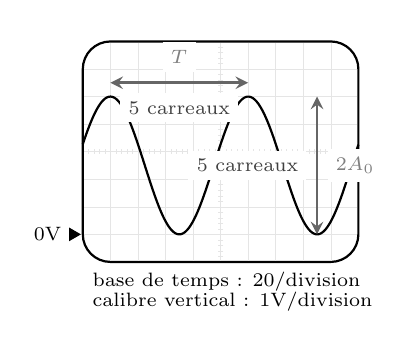
\begin{tikzpicture}[scale=0.35]
	%ecran oscilloscope
	\draw[black,thick,rounded corners=10pt] (0,0) rectangle (10,8) (0.5,-0.5) ;
	\draw (0,0) node[below right] {\scriptsize base de temps : \SI{20}{\micro\second/division}} ;
	\draw (0,-0.75) node[below right] {\scriptsize calibre vertical : \SI{1}{V/division}} ;

		\clip (-2,0.05) rectangle (11,8.5);%créer une découpe de la fenêtre comme indiqué
		\foreach \x in {1,2,...,9}%Démarrage d'une boucle : "pour tout x appartenant à ..."
		{
			%la boucle est délimitée par une paire d'accolade
			\draw[gray!20, very thin] (\x,0.05) -- (\x,7.95);%thin = fin, il existe aussi very thin et ultra thin
		}
		\foreach \y in {1,2,...,7}
		{
			\draw[gray!20, very thin] (0.05,\y) -- (9.95,\y);
		}
		\foreach \x in {0.2,0.4,...,9.8}
		{
			\draw[gray!20, very thin] (\x,4.1) -- (\x,3.9);
		}
		\foreach \y in {0.2,0.4,...,7.8}
		{
			\draw [gray!20, very thin] (5.1,\y) -- (4.9,\y);
		}
		%FIN ecran oscilloscope
		% Les tensions d'entrée et de sortie
		\draw[yshift=4cm,color=black,thick,domain=0:10, smooth, samples=150] plot ({\x},{-0.5+2.5*sin(1.256*\x r+pi/10 r)});
		\draw (-1.7,1) node [right, xshift=-1.5mm]  {\scriptsize \SI{0}{V}};
		%legende
		%un triangle définition de la ligne de masse
		\fill [black] (-0.5,0.75) -- ++(30:0.5) -- ++(150:0.5) --cycle ;
		\draw[color=darkgray!80,line width=1pt,<->,>=stealth] (1,6.5) -- (6,6.5) node [midway, above] {\colorbox{white}{\textcolor{gray}{\scriptsize{$T$}}}} node [midway, below] {\colorbox{white}{\textcolor{darkgray}{\scriptsize{5 carreaux}}}} ;
		\draw[color=darkgray!80,line width=1pt,<->,>=stealth] (8.5,1) -- (8.5,6.) node [midway, right] {\colorbox{white}{\textcolor{gray}{\scriptsize{$2A_0$}}}} node [midway, left] {\colorbox{white}{\textcolor{darkgray}{\scriptsize{5 carreaux}}}} ;
		\end{tikzpicture} 
\shorthandon{:!}
 \end{center}

 % --------------------------------------------------------- %
 \finalisationDuPartageDePage %					
 % --------------------------------------------------------- %
 \end{corrige}

 % ************************************** %


 % ^^^^^^^^^^^^^^^^^^^^^^^^^^^^^^^^^^^^^^ %
 %               Question                 %
 % ^^^^^^^^^^^^^^^^^^^^^^^^^^^^^^^^^^^^^^ %

 \begin{enonce}
 	$U_0$
 \end{enonce}

 \reponse{$\SI{2.5}{V}$}

 \begin{corrige}
 	Nous avons 5 carreaux pour la double amplitude, soit $2U_0=5\times 1 = \SI{5}{V}$. Donc, on a $U_0=\SI{2.5}{V}$.
 \end{corrige}

 % ************************************** %

 % =============================================================================== %
 \finEntrainement
 % =============================================================================== %



 
 % --------------------------------------------------------- %
 %                                                           %
 % -------------------- Partie à droite -------------------- %
 %                                                           %
 \initialisationPartieDroite %
 %                                                           %
 %                                                           %
 \smallskip
 \begin{center}
 	\def\scaleFigure{0.45}
 	\subimport{_images/}{1-5-Signaux_periodique_1-en_CBD_v3.tex}
 \end{center}
 % --------------------------------------------------------- %
 \finalisationDuPartageDePage %					
 % --------------------------------------------------------- %
 
 

\medskip



 % ********************************************************************* %
 %                           ENTRAÎNEMENT                                % 
 % ********************************************************************* %
 % ================ Métadonnées sur l'entraînement ===================== %

 \titreEntrainementFacultatif		{Expression d'une tension}
 \hauteurLargeurCadreReponse		{7mm}{5cm}
 \dureeResolutionFacultative		{1} % 1, 2, 3 ou 4
 \typeEntrainement					{QCM} % Newton ou QCM ou AN ou vide (exercice "normal")
 \basiqueEtTransversal				{Y}
 \nombreColonnesQuestions			{1} % vide, 1, 2, 3, etc.
 \avecPlusieursQuestions			{N} % Y ou N
 \initialisationEntrainement
 % ===================================================================== %


% =============================================================================== %
\debutEntrainement
% =============================================================================== %

% ^^^^^^^^^^^^^^^^^^^^^^^^^^^^^^^^^^^^^^ %
%               Question                 %
% ^^^^^^^^^^^^^^^^^^^^^^^^^^^^^^^^^^^^^^ %
\begin{enonce}
	 Nous disposons d'une tension sinusoïdale $u(t)$ de période $T_0=\SI{1}{ms}$, d'amplitude $U_0=\SI{2}{V}$ et de phase à l'origine $\varphi=\SI{0}{rad}$. 
	
	Parmi les propositions ci-dessous laquelle correspond à l'expression littérale de cette tension $u(t)$ ?
	
	\smallskip

	\begin{listeQCM2Colonnes}
		\item $u(t) = U_0 \cos \left(\frac{t}{T_0} \right)$
		\item $u(t) = \frac{U_0}{2} \cos \left(\frac{2\pi}{T_0} t \right)$
		\item $u(t) = \frac{U_0}{2} \cos \left(\frac{t}{T_0} \right)$
		\item $u(t) = U_0 \cos \left(\frac{2\pi}{T_0} t\right)$
	\end{listeQCM2Colonnes}
	\bigskip
	\medskip
\end{enonce}

\reponse{ \reponseD{}}

% \begin{corrige}
%	La bonne réponse est $u(t)=U_0 \cos \left(\frac{2\pi}{T_0} t\right)$.
%\end{corrige}


 % ************************************** %

 % =============================================================================== %
 \finEntrainement
 % =============================================================================== %





\newpage



% ********************************************************************* %
%                           ENTRAÎNEMENT                                % 
% ********************************************************************* %
% ================ Métadonnées sur l'entraînement ===================== %

\titreEntrainementFacultatif	{Modulation d'amplitude}
\hauteurLargeurCadreReponse		{8mm}{10cm}
\dureeResolutionFacultative		{2} % 1, 2, 3 ou 4
\typeEntrainement				{} % Newton ou QCM ou AN ou vide (exercice "normal")
\nombreColonnesQuestions		{1} % vide, 1, 2, 3, etc.
\avecPlusieursQuestions			{Y} % Y ou N
\basiqueEtTransversal 			{Y}
\initialisationEntrainement
% ===================================================================== %

On considère un signal modulé, de la forme
\[
s(t)= S_0 \cos \big( 2\pi f_p t\big) \times \Big(1+m \cos \left(2\pi f_0 t\right) \Big) \qquad \text{ avec } \quad 
\begin{cases}
0<m<1 \\
f_p>f_0.
\end{cases}
\]

% =============================================================================== %
\debutEntrainement
% =============================================================================== %

% ^^^^^^^^^^^^^^^^^^^^^^^^^^^^^^^^^^^^^^ %
%               Question                 %
% ^^^^^^^^^^^^^^^^^^^^^^^^^^^^^^^^^^^^^^ %

\begin{enonce}
On rappelle que \minusSmallskip
\[
\begin{cases}
\cos \left(a + b\right) = \cos(a) \cos(b) - \sin(a) \sin(b) \\
\cos \left(a - b\right) = \cos(a) \cos(b) + \sin(a) \sin(b).
\end{cases}
\]
\smallskip

En calculant $\cos \left(a + b\right) + \cos \left(a - b\right)$, trouver 
	une formule pour $\cos(a) \cos(b)$.\smallskip\\\mbox{}
\end{enonce}

\reponse{$\frac{1}{2}\cos \left(a + b\right) + \frac{1}{2}\cos \left(a - b\right)$}

\begin{corrige}
On calcule $\cos \left(a + b\right) + \cos \left(a - b\right) =	2 \cos(a) \cos(b)$ et on en déduit la formule
\[
\cos(a) \cos(b) = \frac{1}{2}\cos \left(a + b\right) + \frac{1}{2}\cos \left(a - b\right).
\]
\end{corrige}
% ************************************** %


% ^^^^^^^^^^^^^^^^^^^^^^^^^^^^^^^^^^^^^^ %
%               Question                 %
% ^^^^^^^^^^^^^^^^^^^^^^^^^^^^^^^^^^^^^^ %
	
	\begin{enonce}
	Développer $s(t)$ et faire apparaître des sommes de cosinus. \smallskip\\\mbox{}
	\end{enonce}
	
\reponse{ %
\begin{tabular}{l} 
$S_0 \cos \left(2\pi f_p t \right)$  \\[1mm]
$\qquad+\frac{mS_0}{2} \bigg( \cos \left( 2\pi\left( f_p + f_0 \right) t \right)$ \\[-1mm]
$\qquad\qquad+ \cos \left( 2\pi\left(f_p - f_0 \right) t \right) \bigg)$
\end{tabular}}
	
\begin{corrige}
On calcule :
\begin{align*}
	s(t) 
	&= S_0 \cos \left(2\pi f_p t\right) \left(1+m \cos \left(2\pi f_0 t\right) \right) = S_0 \cos \left(2\pi f_p t\right) + m S_0 \cos \left(2\pi f_p t\right)\cos \left(2\pi f_0 t\right)\\
&= S_0 \cos \left(2\pi f_p t \right) + \frac{mS_0}{2} \Big( \cos \big( 2\pi\left( f_p + f_0 \right) t \big)
	+ \cos \big( 2\pi\left(f_p - f_0 \right) t \big) \Big).
	\end{align*}
\end{corrige}
% ************************************** %

	
	
% =============================================================================== %
\pauseEntrainement
% =============================================================================== %

\bigskip


On constate que le signal $s(t)$ peut s'écrire comme la somme de trois signaux sinusoïdaux d'amplitudes et de fréquences spécifiques. On représente les différentes amplitudes des composantes de $s(t)$ en fonction de leur fréquence. Cette représentation est appelée spectre en amplitude de $s(t)$.

Le but de cet entraînement est de déterminer lequel des spectres ci-dessous (\reponseA{}, \reponseB{} ou \reponseC{}) est celui du signal $s(t)$.


\hauteurLargeurCadreReponse		{7mm}{5.cm}


%Un spectre en amplitude représente les différentes amplitudes des composantes d'un signal en fonction de leur fréquence. 

%Nous souhaitons déterminer le spectre de $s(t)$ obtenu par l'étudiant parmi les trois présentés ci-dessous. 


\begin{center}
	\def\scaleImage{0.55}
	\subimport{_images/}{1-7-Modulation_1_quatre_spectres_CBD_v1.tex}
\end{center} 

% =============================================================================== %
\repriseEntrainement
% =============================================================================== %

% ^^^^^^^^^^^^^^^^^^^^^^^^^^^^^^^^^^^^^^ %
%               Question                 %
% ^^^^^^^^^^^^^^^^^^^^^^^^^^^^^^^^^^^^^^ %

\begin{enonce}
	Donner l'amplitude de la composante de fréquence $f_p$ de $s(t)$
\end{enonce}

\reponse{$S_0$}

\begin{corrige}
	La composante de fréquence $f_p$ de $s(t)$ est $S_0 \cos \left(2 \pi f_p t \right)$, son amplitude est donc de $S_0$.
\end{corrige}

% ************************************** %


% ^^^^^^^^^^^^^^^^^^^^^^^^^^^^^^^^^^^^^^ %
%               Question                 %
% ^^^^^^^^^^^^^^^^^^^^^^^^^^^^^^^^^^^^^^ %

\begin{enonce}
	Donner l'amplitude de la composante de fréquence $f_p + f_0$ de $s(t)$
\end{enonce}

\reponse{$mS_0/2$}

\begin{corrige}
	La composante de fréquence $f_p+f_0$ de $s(t)$ est $\frac{mS_0}{2} \cos \left(2 \pi \left(f_p+f_0\right) t \right)$, son amplitude est donc de $\frac{mS_0}{2}$.
\end{corrige}

% ************************************** %

% ^^^^^^^^^^^^^^^^^^^^^^^^^^^^^^^^^^^^^^ %
%               Question                 %
% ^^^^^^^^^^^^^^^^^^^^^^^^^^^^^^^^^^^^^^ %

\begin{enonce}
	Donner l'amplitude de la composante de fréquence $f_p - f_0$ de $s(t)$
\end{enonce}

\reponse{$mS_0/2$}

\begin{corrige}
	La composante de fréquence $f_p-f_0$ de $s(t)$ est $\frac{mS_0}{2} \cos \left(2 \pi \left(f_p-f_0\right) t \right)$, son amplitude est donc de $\frac{mS_0}{2}$.
\end{corrige}

% ************************************** %

% ^^^^^^^^^^^^^^^^^^^^^^^^^^^^^^^^^^^^^^ %
%               Question                 %
% ^^^^^^^^^^^^^^^^^^^^^^^^^^^^^^^^^^^^^^ %

\begin{enonce}
	Déterminer le spectre (\reponseA{}, \reponseB{} ou \reponseC{})  correspondant à $s(t)$
\end{enonce}

\reponse{$\reponseA{}$}

% \begin{corrige}

% \end{corrige}

% ************************************** %

% =============================================================================== %
\finEntrainement
% =============================================================================== %



\newpage








% ********************************************************************* %
%                           ENTRAÎNEMENT                                % 
% ********************************************************************* %
% ================ Métadonnées sur l'entraînement ===================== %

\titreEntrainementFacultatif	{Pêle-mêle}
\hauteurLargeurCadreReponse		{7mm}{2.5cm}
\dureeResolutionFacultative		{2} % 1, 2, 3 ou 4
\typeEntrainement				{QCM} % Newton ou QCM ou AN ou vide (exercice "normal")
\nombreColonnesQuestions		{2} % vide, 1, 2, 3, etc.
\avecPlusieursQuestions			{Y} % Y ou N
\initialisationEntrainement
% ===================================================================== %

Un étudiant dispose de quatre spectres en amplitude et de quatre signaux. Malheureusement, l'ensemble est mélangé.
Pouvez-vous l'aider à associer le bon signal au bon spectre (\reponseA{}, \reponseB{}, \reponseC{} ou \reponseD{}) ?   
%
%
\begin{center}
	\begin{tabular}{|c|c|}
		\hline	
		 &  \\
		 Spectre $\reponseA{}$ & Spectre $\reponseB{}$\\[2mm]
		\subimport{_images/}{1-9-Spectre-a_CLE_v2.tex} & \subimport{_images/}{1-9-Spectre-b_CLE_v2.tex}\\
		\hline
		 &  \\
		 Spectre $\reponseC{}$ & Spectre $\reponseD{}$\\[2mm]
		\subimport{_images/}{1-9-Spectre-c_CLE_v2.tex} & \subimport{_images/}{1-9-Spectre-d_CLE_v2.tex}\\
		\hline
	\end{tabular}
\end{center} 
%
\begin{center}
	\begin{tabular}{|c|c|}
		\hline	
		  &  \\
		\textbf{Signal \no{}1} &\textbf{Signal \no{}2}\\[2mm]
		  &  \\
		$A_1\left(\cos\left(\omega_0 t\right)+\frac{1}{2}\cos\left(3\omega_0 t\right)+\frac{1}{3}\cos\left(5\omega_0 t\right)\right)$	 & $A_2\left(1+\sin\left(\omega_0 t\right)+\frac{1}{2}\sin\left(2\omega_0 t\right)+\frac{1}{3}\sin\left(3\omega_0 t\right)\right)$
	\\
	  &  \\
			avec $A_1=1$ V et $f_0=1$ kHz & avec $A_2=1$ V et $f_0=2$ kHz \\
			  &  \\
		\hline
		  &  \\
			\textbf{Signal \no{}3} & \textbf{Signal \no{}4}\\[2mm]
		&  \\
		$A_3\Bigl(\cos\left(\left(\omega_0-\omega_1\right) t\right)+\frac{1}{2}\cos\left(\left(\omega_0+\omega_1\right) t\right)$&  $A_4\left(1+\sin\left(\omega_0 t\right)+\frac{1}{2}\sin\left(3\omega_0 t\right)+\frac{1}{3}\sin\left(5\omega_0 t\right)\right)$
		\\
		&  \\
		$\qquad\qquad\qquad\qquad\qquad\qquad{} +\frac{1}{3}\cos\left(\left(\omega_0+3\omega_1\right) t\right)\Bigr)$& \\
		&  \\
		avec $A_3=1$ V, $f_0=3$ kHz et  $f_1=1$ kHz & avec $A_4=1$ V et $f_0=1$ kHz \\
		&  \\
		\hline
	\end{tabular}
\end{center}                       
 %

\smallskip

% =============================================================================== %
\debutEntrainement
% =============================================================================== %
% ^^^^^^^^^^^^^^^^^^^^^^^^^^^^^^^^^^^^^^ %
%               Question                 %
% ^^^^^^^^^^^^^^^^^^^^^^^^^^^^^^^^^^^^^^ %

\begin{enonce}
	Spectre du signal \no{}1
\end{enonce}

\reponse{$\reponseC{}$}

\begin{corrige}
	Nous notons la somme de 3 fonctions sinusoïdales de fréquences respectives $\SI{1}{kHz}$, $\SI{3}{kHz}$ et 
	$\SI{5}{kHz}$. Les spectres \reponseA{} et \reponseD{} ne peuvent pas convenir. 
	
	De plus, la valeur moyenne de $s_1(t)$ est nulle. Le spectre \reponseC{} est donc à associer à $s_1(t)$.
\end{corrige}

% ************************************** %

% ^^^^^^^^^^^^^^^^^^^^^^^^^^^^^^^^^^^^^^ %
%               Question                 %
% ^^^^^^^^^^^^^^^^^^^^^^^^^^^^^^^^^^^^^^ %

\begin{enonce}
	Spectre du signal \no{}2
\end{enonce}

\reponse{$\reponseA{}$}


\begin{corrige}
	Nous notons la somme de 3 fonctions sinusoïdales de fréquences respectives $\SI{2}{kHz}$, $\SI{4}{kHz}$ et $\SI{6}{kHz}$. Les spectres \reponseB{} et \reponseC{} ne peuvent pas convenir. 
	
	De plus, la valeur moyenne de $s_2(t)$ est égale à $\SI{1}{V}$. Le spectre \reponseA{} est donc à associer à  $s_2(t)$.
\end{corrige}

% ************************************** %

% ^^^^^^^^^^^^^^^^^^^^^^^^^^^^^^^^^^^^^^ %
%               Question                 %
% ^^^^^^^^^^^^^^^^^^^^^^^^^^^^^^^^^^^^^^ %

\begin{enonce}
	Spectre du signal \no{}3
\end{enonce}

\reponse{$\reponseD{}$}

\begin{corrige}
	Nous notons la somme de 3 fonctions sinusoïdales de fréquences respectives $\SI{2}{kHz}$, $\SI{4}{kHz}$ et 
	$\SI{6}{kHz}$. Les spectres \reponseB{} et \reponseC{} ne peuvent pas convenir. 
	
	De plus, la valeur moyenne de $s_3(t)$ est nulle. Le spectre \reponseD{} est donc à associer à  $s_3(t)$.
\end{corrige}

% ************************************** %

% ^^^^^^^^^^^^^^^^^^^^^^^^^^^^^^^^^^^^^^ %
%               Question                 %
% ^^^^^^^^^^^^^^^^^^^^^^^^^^^^^^^^^^^^^^ %

\begin{enonce}
	Spectre du signal \no{}4
\end{enonce}

\reponse{$\reponseB{}$}

\begin{corrige}
	Nous notons la somme de 3 fonctions sinusoïdales de fréquences respectives $\SI{1}{kHz}$, $\SI{3}{kHz}$ et 
	$\SI{5}{kHz}$. Les spectres \reponseA{} et \reponseD{} ne peuvent pas convenir. 
	
	De plus, la valeur moyenne de $s_4(t)$ est égale à $\SI{1}{V}$. Le spectre \reponseB{} est donc à associer à  $s_4(t)$.
\end{corrige}

% ************************************** %

% =============================================================================== %
\finEntrainement
% =============================================================================== %







 
% •••••••••••••••••••••••••••••••••••••••••••••••••••••••••••••••••••••••••••• %
% •••••••••••••••••••••••••••••••••••••••••••••••••••••••••••••••••••••••••••• %
\sectionFicheEntrainement{Fonctions de transfert}
% •••••••••••••••••••••••••••••••••••••••••••••••••••••••••••••••••••••••••••• %
% •••••••••••••••••••••••••••••••••••••••••••••••••••••••••••••••••••••••••••• %





% ********************************************************************* %
%                           ENTRAÎNEMENT                                % 
% ********************************************************************* %
% ================ Métadonnées sur l'entraînement ===================== %

\titreEntrainementFacultatif	{Filtre passe-bande}
\hauteurLargeurCadreReponse		{6mm}{3.25cm}
\dureeResolutionFacultative		{3} % 1, 2, 3 ou 4
\typeEntrainement				{Newton} % Newton ou QCM ou AN ou vide (exercice "normal")
\nombreColonnesQuestions		{2} % vide, 1, 2, 3, etc.
\avecPlusieursQuestions			{Y} % Y ou N
\initialisationEntrainement
% ===================================================================== %


%
% mmmmmmmmmmmmmmmmmmmmmmmmmmmmmmmmmmmmmmmmmmmmmmmmmmmmmmmmm %
% 		  Insertion d'une image en regard d'un texte
% mmmmmmmmmmmmmmmmmmmmmmmmmmmmmmmmmmmmmmmmmmmmmmmmmmmmmmmmm %
% --------------------------------------------------------- %
\pourcentageDeLaPartieAGauche   {0.65}
% --------------------------------------------------------- %
%                                                           %
% -------------------- Partie à gauche -------------------- %
\initialisationPartieGauche % 
Nous disposons du filtre ci-contre, constitué de deux dipôles dont les impédances complexes sont :
\[
\underline{Z}_1=R+\frac{1}{\jC C \omega} \quad \text{et} \quad
\underline{Z}_2=\frac{R}{1+\jC RC \omega} \quad \text{avec} \quad C=\SI{47}{nF}  \text{ et }  R=\SI{1}{k\Omega}.
\]

% --------------------------------------------------------- %
%                                                           %
% -------------------- Partie à droite -------------------- %
%                                                           %
\initialisationPartieDroite %
\begin{center}
	\subimport{_images/}{1-10-Filtre_passe_bande-en_CBD_v3.tex}	
\end{center}
% --------------------------------------------------------- %
\finalisationDuPartageDePage %					
% --------------------------------------------------------- %

Nous souhaitons écrire la fonction de transfert du filtre $\underline{H}(\jC \omega) = \frac{\underline{u}_s}{\underline{u}_e}$ sous sa forme canonique :\minusSmallskip
\[
\underline{H}(\jC x)=\frac{H_0}{1+\jC Q\left(x-\frac{1}{x}\right)} \qquad \text{avec} \qquad x=\frac{\omega}{\omega_0}.
\]

\smallskip

% =============================================================================== %
\debutEntrainement
% =============================================================================== %
% ^^^^^^^^^^^^^^^^^^^^^^^^^^^^^^^^^^^^^^ %
%               Question                 %
% ^^^^^^^^^^^^^^^^^^^^^^^^^^^^^^^^^^^^^^ %

\begin{enonce}
À l'aide d'un pont diviseur de tension,\\[1mm]
exprimer $\underline{H}(\jC \omega)$
\end{enonce}

\reponse{$\frac{ \frac{1}{3} }{1+\frac{1}{3\jC RC \omega}+\frac{\jC RC \omega}{3}}$}

\begin{corrige}
    À l'aide d'un pont diviseur de tension, on constate que $
	\underline{u}_s = \underline{u}_e \frac{\underline{Z}_2}{\underline{Z}_1+\underline{Z}_2}
	$. Ainsi, on a
	\begin{align*}
	\underline{H}(\jC \omega) 
	&= \frac{\underline{u}_s}{\underline{u}_e} = \frac{\underline{Z}_2}{\underline{Z}_1+\underline{Z}_2}=
	\frac{R}{1+\jC RC \omega} \frac{ 1 }{ R + \frac{1}{\jC C \omega} + \frac{R}{1 + \jC RC \omega} }
	=\frac{R}{1+\jC RC \omega} \frac{ 1 + \jC RC \omega }{ 3R + \jC R^2C \omega + \frac{1}{\jC C \omega}}\\
	&=	\frac{ R }{ 3R + \jC \left(  R^2C \omega - \frac{1}{C \omega} \right) } 
	=
	\frac{ \frac{1}{3} }{ 1 + \jC \frac{1}{3} \left(  RC \omega - \frac{1}{RC\omega} \right) }.
	\end{align*}
\end{corrige}

% ************************************** %


% ^^^^^^^^^^^^^^^^^^^^^^^^^^^^^^^^^^^^^^ %
%               Question                 %
% ^^^^^^^^^^^^^^^^^^^^^^^^^^^^^^^^^^^^^^ %

\begin{enonce}
	Identifier $H_0$
\end{enonce}

\reponse{$1/3$}

\begin{corrigeNewpage}
    Par identification dans l'expression de $\underline{H}(\jC \omega)$ trouvée précédemment avec la forme canonique, nous en déduisons que $H_0 = \frac{1}{3}$.
\end{corrigeNewpage}

% ************************************** %

% ^^^^^^^^^^^^^^^^^^^^^^^^^^^^^^^^^^^^^^ %
%               Question                 %
% ^^^^^^^^^^^^^^^^^^^^^^^^^^^^^^^^^^^^^^ %

\begin{enonce}
	Identifier $Q$
\end{enonce}

\reponse{$1/3$}

\begin{corrige}
	Par identification dans l'expression de $\underline{H}(\jC \omega)$ trouvée précédemment avec la forme canonique, nous en déduisons que $Q= \frac{1}{3}$.
\end{corrige}

% ************************************** %

% ^^^^^^^^^^^^^^^^^^^^^^^^^^^^^^^^^^^^^^ %
%               Question                 %
% ^^^^^^^^^^^^^^^^^^^^^^^^^^^^^^^^^^^^^^ %

\begin{enonce}
	Identifier et calculer $\omega_0$
\end{enonce}

\reponse{$\SI{2.1e4}{rad/s}$}

\begin{corrige}
	Par identification de l'expression de $\underline{H}(\jC \omega)$ trouvée précédemment avec la forme canonique, nous en déduisons que $x = RC \omega$ donc que $\omega_0= \frac{1}{RC}$. L'application numérique donne
	\[ 
	\omega_0=\frac{1}{RC} = \frac{1}{ \SI{1e3}{\ohm} \times \SI{47e-9}{F} } = \SI{2.1e4}{rad/s}.
	\]
\end{corrige}

% ************************************** %

% =============================================================================== %
\finEntrainement
% =============================================================================== %







% ********************************************************************* %
%                           ENTRAÎNEMENT                                % 
% ********************************************************************* %
% ================ Métadonnées sur l'entraînement ===================== %

\titreEntrainementFacultatif	{Filtre du second ordre}
\hauteurLargeurCadreReponse		{7mm}{6cm}
\dureeResolutionFacultative		{4} % 1, 2, 3 ou 4
\typeEntrainement				{Newton} % Newton ou QCM ou AN ou vide (exercice "normal")
\nombreColonnesQuestions		{1} % vide, 1, 2, 3, etc.
\avecPlusieursQuestions			{Y} % Y ou N
\initialisationEntrainement
% ===================================================================== %


%
% mmmmmmmmmmmmmmmmmmmmmmmmmmmmmmmmmmmmmmmmmmmmmmmmmmmmmmmmm %
% 		  Insertion d'une image en regard d'un texte
% mmmmmmmmmmmmmmmmmmmmmmmmmmmmmmmmmmmmmmmmmmmmmmmmmmmmmmmmm %
% --------------------------------------------------------- %
\pourcentageDeLaPartieAGauche   {0.5}
% --------------------------------------------------------- %
%                                                           %
% -------------------- Partie à gauche -------------------- %
%                                                           %
\initialisationPartieGauche % 
%                                                           %
Nous disposons d'un filtre passe-bas de fonction de transfert : \minusSmallskip
\[
\underline{H}(\jC x)= \frac{\underline{u}_s}{\underline{u}_e} = \frac{H_0}{1+\frac{\jC x}{Q}-x^2} \minusSmallskip
\]
avec $x=\frac{\omega}{\omega_0}$. On a $C=\SI{10}{\micro F}$ et $R=\SI{220}{ \Omega}$.

% --------------------------------------------------------- %
%                                                           %
% -------------------- Partie à droite -------------------- %
%                                                           %
\initialisationPartieDroite %
%                                                           %
%                                                           %                                                      %
\begin{center}
	\subimport{_images/}{1-11-Filtre2nd_ordre_en_CBD_v3.tex}	
\end{center}

% --------------------------------------------------------- %
\finalisationDuPartageDePage %					
% --------------------------------------------------------- %

\minusMedskip

	 Un étudiant obtient les trois égalités suivantes : 
	 \[
	 R\underline{i}  =  \underline{u}_e-\underline{u}, \qquad		
	R\underline{i}_1  =  \underline{u}-\underline{u}_s\qquad \text{et}\qquad 
 		R\underline{i}_2  =  \jC RC\omega \underline{u}.
		\]

\minusBigskip

% =============================================================================== %
\debutEntrainement
% =============================================================================== %

% ^^^^^^^^^^^^^^^^^^^^^^^^^^^^^^^^^^^^^^ %
%               Question                 %
% ^^^^^^^^^^^^^^^^^^^^^^^^^^^^^^^^^^^^^^ %

\hauteurLargeurCadreReponse		{7mm}{3cm}

\begin{enonce}
	À l'aide de la loi des noeuds, exprimer $\underline{i}$ en fonction de $\underline{i}_1$ et $\underline{i}_2$.	
\end{enonce}

\reponse{$\underline{i}_1 + \underline{i}_2$}

\begin{corrige}
D'après la loi des noeuds $\underline{i} = \underline{i}_1 + \underline{i}_2$.
\end{corrige}

% ************************************** %

\hauteurLargeurCadreReponse		{7mm}{6cm}

% ^^^^^^^^^^^^^^^^^^^^^^^^^^^^^^^^^^^^^^ %
%               Question                 %
% ^^^^^^^^^^^^^^^^^^^^^^^^^^^^^^^^^^^^^^ %

\begin{enonce}
	Utiliser la réponse précédente et les trois égalités fournies pour exprimer $\underline{u}_e$ en fonction de $\underline{u}$ et $\underline{u}_s$.\smallskip\\\mbox{}
\end{enonce}

\reponse{$\underline{u} \left( 2 + \jC RC \omega \right) - \underline{u}_s $}

\begin{corrige}
En multipliant la réponse précédente par la résistance $R$, on obtient
$R\underline{i} = R\underline{i}_1 + R\underline{i}_2$. 

Ainsi, d'après les trois égalités, on a
\begin{align*}
	\underline{u}_e - \underline{u} = \underline{u} - \underline{u}_s + \jC RC \omega \underline{u}
	\qquad \text{donc} \qquad
	\underline{u}_e = \underline{u} \left( 2 + \jC RC \omega\right) - \underline{u}_s.
\end{align*}
\end{corrige}

% ************************************** %


% =============================================================================== %
\pauseEntrainement
% =============================================================================== %

\medskip

L'étudiant montre grâce à un pont diviseur de tension que 
\(
\underline{u}=\left(1+\jC RC\omega\right)\underline{u}_s. \minusBigskip
\)

\bigskip


% =============================================================================== %
\repriseEntrainement
% =============================================================================== %


\hauteurLargeurCadreReponse		{8mm}{6cm}


% ^^^^^^^^^^^^^^^^^^^^^^^^^^^^^^^^^^^^^^ %
%               Question                 %
% ^^^^^^^^^^^^^^^^^^^^^^^^^^^^^^^^^^^^^^ %

\begin{enonce}
 	En déduire la fonction de transfert simplifiée $\underline{H}(\jC \omega)$.	
\end{enonce}

\reponse{$\frac{1}{1+3\jC RC\omega -\left(RC\omega\right)^2}$}

\begin{corrige}
	En utilisant la réponse précédente et en exprimant $\underline{u}$ à partir de la relation donnée, il vient que
\[
	\underline{u}_e = \underline{u}_s \left(1+\jC RC\omega\right) \left( 2 + \jC RC \omega\right) - \underline{u}_s = \underline{u}_s \left( 1 + 3\jC RC \omega  - \left(RC \omega \right)^2 \right).
	\]
	Ainsi, on a $\underline{H}(\jC \omega) = \frac{\underline{u}_s}{\underline{u}_e}
		= \frac{1}{ 1 + 3\jC RC \omega  - \left(RC \omega \right)^2}$.
\end{corrige}

% ************************************** %


% =============================================================================== %
\pauseEntrainement
% =============================================================================== %
\bigskip

En comparant la réponse précédente à la forme canonique de $\underline{H}(\jC\omega)$ donnée, identifier 

\smallskip
% =============================================================================== %
\repriseEntrainement
% =============================================================================== %

\enlargethispage{1cm}
\hauteurLargeurCadreReponse		{7mm}{2cm}
\begin{multicols}{3}

% ^^^^^^^^^^^^^^^^^^^^^^^^^^^^^^^^^^^^^^ %
%               Question                 %
% ^^^^^^^^^^^^^^^^^^^^^^^^^^^^^^^^^^^^^^ %

\begin{enonce}
	$H_0$
\end{enonce}
\
\reponse{$1$}

\begin{corrige}
	En comparant les deux égalités
\[
	\underline{H}(\jC \omega) =\frac{H_0}{1+\frac{\jC x}{Q}-x^2} \qquad \text{et} \qquad
	\underline{H}(\jC \omega)= \frac{1}{ 1 + 3\jC RC \omega  - \left(RC \omega \right)^2 }
	\]
	on trouve $H_0 = 1 $ et $x = \frac{\omega}{\omega_0} = RC \omega$ donc $\omega_0 = \frac{1}{RC}$ et  $Q = \frac{1}{3}$.
\end{corrige}

% ************************************** %

% ^^^^^^^^^^^^^^^^^^^^^^^^^^^^^^^^^^^^^^ %
%               Question                 %
% ^^^^^^^^^^^^^^^^^^^^^^^^^^^^^^^^^^^^^^ %

\begin{enonce}
	$\omega_0$
\end{enonce}

\reponse{$\frac{1}{RC}$}

%\begin{corrige}
%
%\end{corrige}
% ************************************** %

% ^^^^^^^^^^^^^^^^^^^^^^^^^^^^^^^^^^^^^^ %
%               Question                 %
% ^^^^^^^^^^^^^^^^^^^^^^^^^^^^^^^^^^^^^^ %

\begin{enonce}
	$Q$
\end{enonce}

\reponse{$1/3$}

%\begin{corrige}
%
%\end{corrige}
% ************************************** %

\end{multicols}

% =============================================================================== %
\finEntrainement
% =============================================================================== %


\newpage



% •••••••••••••••••••••••••••••••••••••••••••••••••••••••••••••••••••••••••••• %
% •••••••••••••••••••••••••••••••••••••••••••••••••••••••••••••••••••••••••••• %
\sectionFicheEntrainement{De la fonction de transfert au diagramme de Bode}
% •••••••••••••••••••••••••••••••••••••••••••••••••••••••••••••••••••••••••••• %
% •••••••••••••••••••••••••••••••••••••••••••••••••••••••••••••••••••••••••••• %



% ********************************************************************* %
%                           ENTRAÎNEMENT                                % 
% ********************************************************************* %
% ================ Métadonnées sur l'entraînement ===================== %

\titreEntrainementFacultatif	{Calcul de gain en décibel}
\hauteurLargeurCadreReponse		{6mm}{5cm}
\dureeResolutionFacultative		{1} % 1, 2, 3 ou 4
\typeEntrainement				{Newton} % Newton ou QCM ou AN ou vide (exercice "normal")
\nombreColonnesQuestions		{2} % vide, 1, 2, 3, etc.
\avecPlusieursQuestions			{Y} % Y ou N
\basiqueEtTransversal {Y}
\initialisationEntrainement
% ===================================================================== %

On considère les fonctions de transfert suivantes : 
$\underline{H}_1=\np{3,0}$ et  $\underline{H}_2=\jC \frac{ \omega}{\omega_0}$ et $\underline{H}_3=1+ \jC \frac{ \omega}{\omega_1}$.


Le gain en décibel $G_{\text{dB}}$ d'un filtre se détermine à partir de la relation : 
\[
	G_{\text{dB}}= 20 \log\big(\, \left | \underline{H}\right|\,  \big).
\]
Déterminer le gain en décibel associé aux différentes fonctions de transfert ou combinaisons de fonctions de transfert ci-dessous.

% =============================================================================== %
\debutEntrainement
% =============================================================================== %

% ^^^^^^^^^^^^^^^^^^^^^^^^^^^^^^^^^^^^^^ %
%               Question                 %
% ^^^^^^^^^^^^^^^^^^^^^^^^^^^^^^^^^^^^^^ %

\begin{enonce}
	$\underline{H}_1$
\end{enonce}

\reponse{$\SI{9,5}{dB}$}

\begin{corrige}
On a $G_{\text{dB}_{1}}=20\log\left(\lVert 3  \rVert \right)=20\log\left( 3  \right)=\SI{9,5}{dB}$.
\end{corrige}

% ************************************** %


% ^^^^^^^^^^^^^^^^^^^^^^^^^^^^^^^^^^^^^^ %
%               Question                 %
% ^^^^^^^^^^^^^^^^^^^^^^^^^^^^^^^^^^^^^^ %

\begin{enonce}
	$\underline{H}_2$
\end{enonce}

\reponse{$20\log\left(\frac{\omega}{\omega_0}\right) $}

\begin{corrige}
	On a $G_{\text{dB}_{2}}
	=20\log\left(\left|  \jC \frac{ \omega}{\omega_0} \right| \right)
	=20\log\left( \frac{ \omega}{\omega_0}  \right)$.	
\end{corrige}

% ************************************** %


% ^^^^^^^^^^^^^^^^^^^^^^^^^^^^^^^^^^^^^^ %
%               Question                 %
% ^^^^^^^^^^^^^^^^^^^^^^^^^^^^^^^^^^^^^^ %

\begin{enonce}
	$\underline{H}_3$
\end{enonce}

\reponse{	$10\log\left(1+\left( \frac{\omega}{\omega_1} \right)^2\right) $}
	
\begin{corrige}
On calcule \minusSmallskip
		\begin{align*}
		G_{\text{dB}_{3}} &=20\log\left(\left| 1+\jC \frac{\omega}{\omega_1} \right| \right)=20\log\left(\sqrt{1+ \left( \frac{\omega}{\omega_1} \right)^2}\right) = 20\log\left(\left( 1+ \left( \frac{\omega}{\omega_1} \right)^2\right)^{\frac{1}{2}} \right)\\
		&= 20 \times \frac{1}{2} \log\left( 1+ \left( \frac{\omega}{\omega_1} \right)^2\right) =  10\log\left( 1+ \left( \frac{\omega}{\omega_1} \right)^2\right).
		\end{align*}
\end{corrige}

% ************************************** %


% ^^^^^^^^^^^^^^^^^^^^^^^^^^^^^^^^^^^^^^ %
%               Question                 %
% ^^^^^^^^^^^^^^^^^^^^^^^^^^^^^^^^^^^^^^ %

\begin{enonce}
	$\underline{H}_1-\underline{H}_2$
\end{enonce}

\reponse{$10 \log\left(9+\left( \frac{\omega}{\omega_0} \right)^2\right)$}

\begin{corrigeNewpage}
	On a 
	\[
	G_{\text{dB}_{4}} =20\log\left(\left| \underline{H}_1-\underline{H}_2 \right| \right)
		= 20\log\left(\left| 3-\jC \frac{ \omega}{\omega_0} \right| \right) = 20\log\left(\sqrt{9+\left( \frac{\omega}{\omega_0} \right)^2}\right) = 10 \log\left(9+\left( \frac{\omega}{\omega_0} \right)^2\right).
		\]
\end{corrigeNewpage}

% ************************************** %


% ^^^^^^^^^^^^^^^^^^^^^^^^^^^^^^^^^^^^^^ %
%               Question                 %
% ^^^^^^^^^^^^^^^^^^^^^^^^^^^^^^^^^^^^^^ %

\begin{enonce}
	$\frac{\underline{H}_2}{\underline{H}_3}$
\end{enonce}

\reponse{	$20\log\left(\frac{\omega}{\omega_0}\right) - 10\log\left( 1+ \left( \frac{\omega}{\omega_1} \right)^2\right)$}

\begin{corrige}
On calcule 
	\begin{align*}
	G_{\text{dB}_{5}} &=20\log\left(\left| \frac{\underline{H}_2}{\underline{H}_3} \right| \right)
	= 20\log\left( \frac{\left| \underline{H}_2 \right|}{ \left| \underline{H}_3 \right|}  \right)
	= 20\log\left( \left| \underline{H}_2 \right| \right) - 20 \log \left( \left| \underline{H}_3 \right|  \right) = G_{\text{dB}_{2}} - G_{\text{dB}_{3}}\\
	&= 20\log\left(\frac{\omega}{\omega_0}\right) - 10\log\left( 1+ \left( \frac{\omega}{\omega_1} \right)^2\right).
	\end{align*}
\end{corrige}

% ************************************** %


% ^^^^^^^^^^^^^^^^^^^^^^^^^^^^^^^^^^^^^^ %
%               Question                 %
% ^^^^^^^^^^^^^^^^^^^^^^^^^^^^^^^^^^^^^^ %

\begin{enonce}
	$\underline{H}_2 \times \underline{H}_3$
\end{enonce}

\reponse{$20\log\left(\frac{\omega}{\omega_0}\right) + 10\log\left( 1+ \left( \frac{\omega}{\omega_1} \right)^2\right)$}

\begin{corrige}
On calcule	
	\begin{align*}
		\hspace{1cm}
		G_{\text{dB}_{6}} &=20\log\left(\left|\underline{H}_2 \times \underline{H}_3 \right| \right)
		= 20\log\left( \left| \underline{H}_2 \right| \times \left| \underline{H}_3 \right|  \right)
		= 20\log\left( \left| \underline{H}_2 \right| \right) + 20 \log \left( \left| \underline{H}_3 \right|  \right) = G_{\text{dB}_{2}} + G_{\text{dB}_{3}}\\
		&= 20\log\left(\frac{\omega}{\omega_0}\right) + 10\log\left( 1+ \left( \frac{\omega}{\omega_1} \right)^2\right).
		\end{align*}
\end{corrige}

% ************************************** %

% =============================================================================== %
\finEntrainement
% =============================================================================== %





% ********************************************************************* %
%                           ENTRAÎNEMENT                                % 
% ********************************************************************* %
% ================ Métadonnées sur l'entraînement ===================== %

\titreEntrainementFacultatif	{Calcul de phase}
\hauteurLargeurCadreReponse		{7mm}{5cm}
\dureeResolutionFacultative		{2} % 1, 2, 3 ou 4
\typeEntrainement				{Newton} % Newton ou QCM ou AN ou vide (exercice "normal")
\nombreColonnesQuestions		{2} % vide, 1, 2, 3, etc.
\avecPlusieursQuestions			{Y} % Y ou N
\basiqueEtTransversal {Y}
\initialisationEntrainement
% ===================================================================== %

On reprend les mêmes fonctions de transfert que précédemment : 
$
 \underline{H}_1=\np{3,0}$ et   $ \underline{H}_2=\jC \frac{ \omega}{\omega_0} $ et $   \underline{H}_3=1+ \jC\frac{ \omega}{\omega_1}
$.


Le déphase $\varphi$ introduit par un filtre entre les signaux d'entrée et de sortie se détermine à partir de la relation : 
\[
\varphi= \arg\left(\underline{H}\right)=\arctan\left(\frac{\Im(\underline{H})}{\Re(\underline{H})}\right).
\]
Déterminer le déphasage associé aux différentes fonctions de transfert ou combinaisons de fonctions de transfert ci-dessous.

% =============================================================================== %
\debutEntrainement
% =============================================================================== %

% ^^^^^^^^^^^^^^^^^^^^^^^^^^^^^^^^^^^^^^ %
%               Question                 %
% ^^^^^^^^^^^^^^^^^^^^^^^^^^^^^^^^^^^^^^ %

\begin{enonce}
	$\underline{H}_1$
\end{enonce}

\reponse{$0$}

\begin{corrige}
On a $\varphi_1= \arg\left( \underline{H}_1 \right) =\arctan \left(  \frac{ \Im\left( \underline{H}_1\right) }{ \Re\left( \underline{H}_1\right) } \right) = \arctan \left(  \frac{ 0 }{ 3 } \right) = \arctan(0) = 0$.
\end{corrige}

% ************************************** %

% ^^^^^^^^^^^^^^^^^^^^^^^^^^^^^^^^^^^^^^ %
%               Question                 %
% ^^^^^^^^^^^^^^^^^^^^^^^^^^^^^^^^^^^^^^ %

\begin{enonce}
	$\underline{H}_2$
\end{enonce}

\reponse{$\pi/2$}
\begin{corrige}
On a $\varphi_2= \arg\left( \underline{H}_2 \right) =\arctan \left(  \frac{ \Im\left( \underline{H}_2\right) }{ \Re\left( \underline{H}_2\right) } \right) = \arctan \left(  \frac{ \frac{\omega}{\omega_0} }{ 0 } \right) = \lim_{x \rightarrow +\infty} \arctan(x) = \frac{\pi}{2}$.
\end{corrige}

% ************************************** %

% ^^^^^^^^^^^^^^^^^^^^^^^^^^^^^^^^^^^^^^ %
%               Question                 %
% ^^^^^^^^^^^^^^^^^^^^^^^^^^^^^^^^^^^^^^ %

\begin{enonce}
	$\underline{H}_3$
\end{enonce}

\reponse{$\arctan \left( \frac{\omega}{\omega_1}  \right)$}

\begin{corrige}
On a $\varphi_3= \arg\left( \underline{H}_3 \right) = \arctan \left(  \frac{ \Im\left( \underline{H}_3\right) }{ \Re\left( \underline{H}_3\right) } \right) = \arctan \left(  \frac{ \frac{\omega}{\omega_1} }{ 1 } \right)
	=\arctan \left( \frac{\omega}{\omega_1}  \right)$.
\end{corrige}

% ************************************** %

% ^^^^^^^^^^^^^^^^^^^^^^^^^^^^^^^^^^^^^^ %
%               Question                 %
% ^^^^^^^^^^^^^^^^^^^^^^^^^^^^^^^^^^^^^^ %

\begin{enonce}
	$\underline{H}_1-\underline{H}_2$
\end{enonce}

\reponse{$-\arctan\left(\frac{\omega}{3\omega_0}\right)$}

\begin{corrige}
On a
$\varphi_4= \arg\left( \underline{H}_1-\underline{H}_2 \right)= \arg\left( 3-\jC \frac{\omega}{\omega_0} \right) = \arctan\left(\frac{-\frac{ \omega}{\omega_0} }{ 3 }\right) = \arctan\left(-\frac{\omega}{ 3\omega_0 }\right) = -\arctan\left(\frac{\omega}{ 3\omega_0 }\right)$.
\end{corrige}

% ************************************** %

% ^^^^^^^^^^^^^^^^^^^^^^^^^^^^^^^^^^^^^^ %
%               Question                 %
% ^^^^^^^^^^^^^^^^^^^^^^^^^^^^^^^^^^^^^^ %

\begin{enonce}
	$\frac{\underline{H}_2}{\underline{H}_3}$
\end{enonce}

\reponse{$\frac{\pi}{2}-\arctan\left(\frac{\omega}{\omega_1}\right)$}

\begin{corrige}
On a $\varphi_5= \arg\left( \frac{\underline{H}_2}{\underline{H}_3} \right)= \arg\left( \underline{H}_2 \right) - \arg\left( \underline{H}_3 \right)
	= \frac{\pi}{2} - \arctan \left( \frac{\omega}{\omega_1}  \right)$.
\end{corrige}

% ************************************** %

% ^^^^^^^^^^^^^^^^^^^^^^^^^^^^^^^^^^^^^^ %
%               Question                 %
% ^^^^^^^^^^^^^^^^^^^^^^^^^^^^^^^^^^^^^^ %

\begin{enonce}
	$\underline{H}_2\times\underline{H}_3$
\end{enonce}

\reponse{$\frac{\pi}{2}+\arctan\left(\frac{\omega}{\omega_1}\right)$}

\begin{corrige}
On a $\varphi_6= \arg\left( \underline{H}_2 \times \underline{H}_3 \right)= \arg\left( \underline{H}_2 \right) + \arg\left( \underline{H}_3 \right)
	= \frac{\pi}{2} + \arctan \left( \frac{\omega}{\omega_1}  \right)$.
\end{corrige}

% ************************************** %

% =============================================================================== %
\finEntrainement
% =============================================================================== %




% ********************************************************************* %
%                           ENTRAÎNEMENT                                % 
% ********************************************************************* %
% ================ Métadonnées sur l'entraînement ===================== %

\titreEntrainementFacultatif	{Diagramme de Bode en phase}
\hauteurLargeurCadreReponse		{6mm}{6cm}
\dureeResolutionFacultative		{1} % 1, 2, 3 ou 4
\typeEntrainement				{AN} % Newton ou QCM ou AN ou vide (exercice "normal")
\basiqueEtTransversal			{Y}
\nombreColonnesQuestions		{1} % vide, 1, 2, 3, etc.
\avecPlusieursQuestions			{Y} % Y ou N
\initialisationEntrainement
% ===================================================================== %

On utilise un filtre passe-haut de fonction de transfert $\underline{H}(\jC x)=\frac{\jC x}{1+\jC x}$ avec $x=\frac{\omega}{\omega_0}$.

Déterminer la valeur du déphasage $\varphi(x) = \arg \Big( \underline{H}(\jC x) \Big)$ du filtre pour des signaux tels que :

% =============================================================================== %
\debutEntrainement
% =============================================================================== %

% ^^^^^^^^^^^^^^^^^^^^^^^^^^^^^^^^^^^^^^ %
%               Question                 %
% ^^^^^^^^^^^^^^^^^^^^^^^^^^^^^^^^^^^^^^ %

\begin{enonce}
	 $\omega = \omega_0$ (la pulsation propre du filtre)
\end{enonce}

\reponse{$\pi/4$}

\begin{corrige}
	Notons que $x = \frac{\omega}{\omega_0} > 0$. Ainsi, on a
	\[
		\varphi = \arg\left(\underline{H}\left(\jC\omega \right) \right)
		= \arg\left( \frac{\jC x}{1 + \jC x} \right)
		=\arg\left(\jC x\right) - \arg\left(1+\jC x\right)
		=\arctan\left( \frac{x}{0} \right) - \arctan\left( \frac{x}{1} \right)
		=\frac{\pi}{2} -\arctan(x).
	\]
	Pour $x=1$, on obtient $\varphi = \frac{\pi}{2} -\arctan(1) = \frac{\pi}{2} - \frac{\pi}{4} = \frac{\pi}{4}$.
\end{corrige}

% ************************************** %

% ^^^^^^^^^^^^^^^^^^^^^^^^^^^^^^^^^^^^^^ %
%               Question                 %
% ^^^^^^^^^^^^^^^^^^^^^^^^^^^^^^^^^^^^^^ %

\begin{enonce}
	$\omega \gg \omega_0$ (en hautes fréquences) 
\end{enonce}

\reponse{$0$}

\begin{corrige}
	On a vu précédemment que $\varphi=\frac{\pi}{2} - \arctan(x)$, ainsi pour $\omega \gg \omega_0$, soit $x \rightarrow +\infty$, il vient que
\[
	\varphi = \lim_{x \rightarrow +\infty} \frac{\pi}{2} - \arctan(x) = \frac{\pi}{2} - \frac{\pi}{2} = 0.
\]
\end{corrige}

% ************************************** %

% ^^^^^^^^^^^^^^^^^^^^^^^^^^^^^^^^^^^^^^ %
%               Question                 %
% ^^^^^^^^^^^^^^^^^^^^^^^^^^^^^^^^^^^^^^ %

\begin{enonce}
	$\omega \ll \omega_0$ (en basses fréquences)
\end{enonce}

\reponse{$\frac{\pi}{2}$}

\begin{corrigeNewpage}
	On a vu précédemment que $\varphi=\frac{\pi}{2} -\arctan(x)$, ainsi pour $\omega \ll \omega_0$, soit $x \rightarrow 0$, il vient que
\[
	\varphi = \frac{\pi}{2} -\arctan(0) = \frac{\pi}{2}.
\]
\end{corrigeNewpage}
% ************************************** %

% =============================================================================== %
\finEntrainement
% =============================================================================== %







% ********************************************************************* %
%                           ENTRAÎNEMENT                                % 
% ********************************************************************* %
% ================ Métadonnées sur l'entraînement ===================== %

\titreEntrainementFacultatif	{Calcul de gain}
\hauteurLargeurCadreReponse		{6mm}{8cm}
\dureeResolutionFacultative		{1} % 1, 2, 3 ou 4
\typeEntrainement				{AN} % Newton ou QCM ou AN ou vide (exercice "normal")
\basiqueEtTransversal			{Y}
\nombreColonnesQuestions		{1} % vide, 1, 2, 3, etc.
\avecPlusieursQuestions			{Y} % Y ou N
\initialisationEntrainement
% ===================================================================== %

Pour les fonctions de transfert suivantes, évaluer le gain $G(x) = \big| \underline{H}\left(\jC x \right) \big|$ pour $x = 1$.

% =============================================================================== %
\debutEntrainement
% =============================================================================== %


% ^^^^^^^^^^^^^^^^^^^^^^^^^^^^^^^^^^^^^^ %
%               Question                 %
% ^^^^^^^^^^^^^^^^^^^^^^^^^^^^^^^^^^^^^^ %

\begin{enonce}
	$\underline{H}\left(\jC x \right)=\frac{1-\jC x}{1+\jC x}$
\end{enonce}

\reponse{$1$}

\begin{corrige}
	Pour $x=1$, $\underline{H}\left(\jC x \right)=\frac{1-\jC}{1+\jC}$, donc
	$
	G(x)= \left| \frac{1-\jC}{1+\jC} \right|
	= \frac{\left| 1-\jC \right|}{\left| 1+\jC \right|} = \frac{\sqrt{1 + 1} }{\sqrt{1 + 1} } = 1
	$.
\end{corrige}

% ************************************** %


% ^^^^^^^^^^^^^^^^^^^^^^^^^^^^^^^^^^^^^^ %
%               Question                 %
% ^^^^^^^^^^^^^^^^^^^^^^^^^^^^^^^^^^^^^^ %

\begin{enonce}
	$\underline{H}\left(\jC x \right)=-\frac{\jC x}{1+\jC x}$
\end{enonce}

\reponse{$1/\sqrt{2}$}

\begin{corrige}
	Pour $x=1$, $\underline{H}\left(\jC x \right)=-\frac{\jC}{1+\jC}$, donc
	$
	G(x)= \left| -\frac{\jC}{1+\jC} \right|
	= \frac{\left| \jC \right|}{\left| 1+\jC \right|} = \frac{1 }{\sqrt{1 + 1} } = \frac{1}{\sqrt{2}}
	$.
\end{corrige}

% ************************************** %


% ^^^^^^^^^^^^^^^^^^^^^^^^^^^^^^^^^^^^^^ %
%               Question                 %
% ^^^^^^^^^^^^^^^^^^^^^^^^^^^^^^^^^^^^^^ %

\begin{enonce}
	$\underline{H}\left(\jC x \right)=\frac{1}{1+2\jC mx+\left(\jC x\right)^2}$ avec $m=2$
\end{enonce}

\reponse{$1/4$}

\begin{corrige}
	Pour $x=1$ et $m=2$, $\underline{H}\left(\jC x \right)=\frac{1}{1+4\jC +\left(\jC \right)^2} = \frac{1}{4\jC}$, donc
	$
	G(x)= \left| \frac{1}{4\jC} \right|
	= \frac{\left| 1 \right|}{\left| 4\jC \right|} = \frac{1}{4}
	$.
\end{corrige}

% ************************************** %

% =============================================================================== %
\finEntrainement
% =============================================================================== %






% ********************************************************************* %
%                           ENTRAÎNEMENT                                % 
% ********************************************************************* %
% ================ Métadonnées sur l'entraînement ===================== %

\titreEntrainementFacultatif	{Tracé sur papier semi-logarithmique}
\hauteurLargeurCadreReponse		{7mm}{2,5cm}
\dureeResolutionFacultative		{1} % 1, 2, 3 ou 4
\typeEntrainement				{AN} % Newton ou QCM ou AN ou vide (exercice "normal")
\nombreColonnesQuestions		{1} % vide, 1, 2, 3, etc.
\avecPlusieursQuestions			{Y} % Y ou N
\initialisationEntrainement
% ===================================================================== %

Un élève souhaite étudier le comportement d'un filtre passe-haut en basses fréquences. Pour cela, il relève les amplitudes des tensions d'entrée et de sortie pour différentes fréquences bien inférieures à la fréquence de coupure du filtre. 
\begin{center}
\renewcommand{\arraystretch}{1.2}
	\begin{tabular}{| p{8cm}| p{1.5cm} |p{1.5cm}|p{1.5cm}|}
		\hline
		\textbf{Fréquence} (en \si{Hz})&  $\np{200}$  &   $\np{700}$  &   $\np{2000}$    \\
			\hline	
		\textbf{Amplitude du signal d'entrée}  ($U_{\text{entrée}}$ en \si{V})  &    $\np{1}$	&      $\np{1}$   &     $\np{1}$      \\
			\hline	
			\textbf{Amplitude du signal de sortie}  ($U_{\text{sortie}}$ en \si{V})  &    $\np{0,04}$	&     $\np{0,14}$   &    $\np{0,40}$      \\
			\hline	
			%Gain en dB ($G_{\text{dB}}$ en dB)  &    	&      &        \\
%\hline	
	\end{tabular}
	\renewcommand{\arraystretch}{1}
\end{center}
%
\begin{center}
	\subimport{_images/}{1-16-papier_semi_log_CBD_v4.tex}
\end{center}
%

Le gain en décibel est donnée par la relation $G_{\text{dB}}=20 \log \left(\frac{U_{\text{sortie}}}{U_{\text{entrée}}}\right)$.

Calculer le gain en décibel pour chacune des fréquences et placer le point correspondant sur le graphe ci-dessus.

% =============================================================================== %
\debutEntrainement
% =============================================================================== %

% ^^^^^^^^^^^^^^^^^^^^^^^^^^^^^^^^^^^^^^ %
%               Question                 %
% ^^^^^^^^^^^^^^^^^^^^^^^^^^^^^^^^^^^^^^ %

\begin{enonce}
	Point $\ptA$ : $f = \SI{200}{Hz}$. 
\end{enonce}

\reponse{$\SI{-28,0}{dB}$}

\begin{corrige}
		On a $G_{\text{dB}} = 20 \log \left(\frac{\np{0,04}}{1}\right)=\SI{-28,0}{dB}$.
\end{corrige}

% ************************************** %

% ^^^^^^^^^^^^^^^^^^^^^^^^^^^^^^^^^^^^^^ %
%               Question                 %
% ^^^^^^^^^^^^^^^^^^^^^^^^^^^^^^^^^^^^^^ %

\begin{enonce}
	Point $\ptB$ : $f = \SI{700}{Hz}$. 
\end{enonce}

\reponse{$\SI{-17,1}{dB}$}

\begin{corrige}
	On a $G_{\text{dB}} = 20 \log \left(\frac{\np{0,14}}{1}\right)=\SI{-17,1}{dB}$.
\end{corrige}

% ************************************** %

% ^^^^^^^^^^^^^^^^^^^^^^^^^^^^^^^^^^^^^^ %
%               Question                 %
% ^^^^^^^^^^^^^^^^^^^^^^^^^^^^^^^^^^^^^^ %

\begin{enonce}
	Point $\ptC$ : $f = \SI{2000}{Hz}$.
\end{enonce}

\reponse{$\SI{-8,0}{dB}$}

\begin{corrige}
	On a $G_{\text{dB}} = 20 \log \left(\frac{\np{0,4}}{1}\right)=\SI{-8,0}{dB}$.
\end{corrige}

% ************************************** %

% ^^^^^^^^^^^^^^^^^^^^^^^^^^^^^^^^^^^^^^ %
%               Question                 %
% ^^^^^^^^^^^^^^^^^^^^^^^^^^^^^^^^^^^^^^ %

\begin{enonce}
	Déterminer la pente de la droite passant les points $\ptA$, $\ptB$ et $\ptC$.
\end{enonce}

\reponse{$+\SI{20}{dB/décade}$}

\begin{corrige}
	Si on mène l'application numérique, la pente $a$ de la droite est
	\[
		a = \frac{ G_{\text{dB}}(\ptC) - G_{\text{dB}}(\ptA) }{ \log\left( f(\ptC) \right) - \log\left( f(\ptA) \right)}
		= \frac{\SI{-8,0}{dB} + \SI{28,0}{dB}}{ \log(2000) - \log(200) } = \SI{20}{dB}.
	\]

% mmmmmmmmmmmmmmmmmmmmmmmmmmmmmmmmmmmmmmmmmmmmmmmmmmmmmmmmm %
% 		  Insertion d'une image en regard d'un texte
% mmmmmmmmmmmmmmmmmmmmmmmmmmmmmmmmmmmmmmmmmmmmmmmmmmmmmmmmm %
% --------------------------------------------------------- %
\pourcentageDeLaPartieAGauche   {0.4}
% --------------------------------------------------------- %
%                                                           %
% -------------------- Partie à gauche -------------------- %
%                                                           %
\initialisationPartieGauche % 
%                                                           % 

Donc, le gain du filtre augmente de \SI{20}{dB} lorsque $\log(f)$ augmente d'une unité, soit lorsque la fréquence $f$ est multipliée par $10$, soit lorsque $f$ augmente d'une décade.

La pente de la droite  $(\ptA\ptC)$  observée sur le graphe est bien de $+\SI{20}{dB/décade}$.


% --------------------------------------------------------- %
%                                                           %
% -------------------- Partie à droite -------------------- %
%                                                           %
\initialisationPartieDroite %
%                                                           %
%  

\begin{center}
	\shorthandoff{:!} %règle un problème de compatibilité avec babel
%
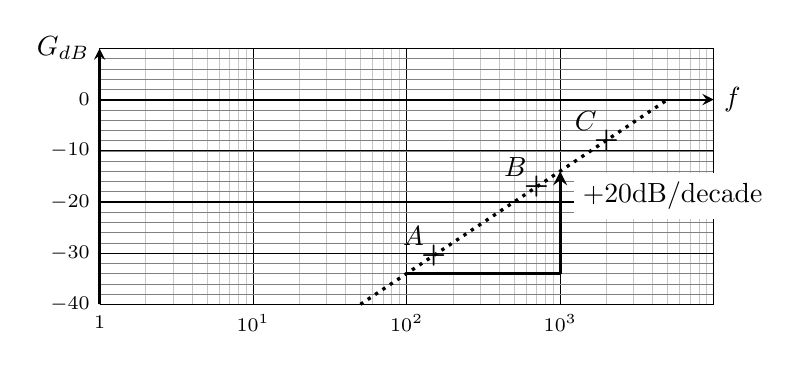
\begin{tikzpicture}[scale=0.65,rotate=0]
	% Dimensions du repere
	\def\xlrg{12} \def\ylrg{5}
%
% Tracé de l'axe log base 10
	\foreach \ee in{0,1,2,3}{
		\foreach \x in {1,2,...,10} {
			\draw[very thin,color=gray!45] ({\xlrg/4*ln(\x*10^\ee)/ln(10)-\xlrg},0)--({\xlrg/4*ln(\x*10^\ee)/ln(10)-\xlrg},-\ylrg);
		};
	};
%tracé de la légende pour les puissances de 10
	\foreach \ee in{1,2,3}{
	\foreach \x in {10}
	{\draw[thin,color=black]({\xlrg/4*ln(\x^\ee)/ln(10)-\xlrg},0)--({\xlrg/4*ln(\x^\ee)/ln(10)-\xlrg},-\ylrg) node [below] {\scriptsize $10^{\ee}$};
	};
	};
% Grille lineaire
	\draw [xstep=\xlrg,ystep=.2,gray,very thin] (-\xlrg,-\ylrg) grid (0,0);  
	\foreach \ee in{-40,-30,...,0}{\draw [color=black](0,{-\ylrg+(\ee+40)/10})(-\xlrg,{-\ylrg+(\ee+40)/10}) node [left] {\scriptsize $\ee$};
	};
	\draw [xstep=\xlrg,ystep=1,color=black] (-\xlrg,-\ylrg) grid (0,0);
%
	% Légende des axes
	\draw[->,>=stealth, thick] (-\xlrg,-1) -- (0,-1) node[right] {$f$};
	\draw[thick, ->,>=stealth] (-\xlrg,-\ylrg) -- (-\xlrg,0) node[left] {$G_{\si{dB}}$};
	\node at (-\xlrg,-\ylrg-0.35) {\scriptsize $1$};
	\draw ({\xlrg/4*ln(150)/ln(10)-\xlrg},-4.04) node  {\textbf{+}}node [above left] {$A$}; ;
	\draw ({\xlrg/4*ln(700)/ln(10)-\xlrg},-2.7) node {\textbf{+}} node [above left] {$B$};
	\draw ({\xlrg/4*ln(2000)/ln(10)-\xlrg},-1.8) node {\textbf{+}} node [above left] {$C$};
	\draw [dotted,very thick]({\xlrg/4*ln(50)/ln(10)-\xlrg},-5)--({\xlrg/4*ln(5000)/ln(10)-\xlrg},-1);
	\draw [very thick]({\xlrg/4*ln(100)/ln(10)-\xlrg},-4.4)--({\xlrg/4*ln(1000)/ln(10)-\xlrg},-4.4);
	\draw [->,>=stealth,very thick] ({\xlrg/4*ln(1000)/ln(10)-\xlrg},-4.4)--({\xlrg/4*ln(1000)/ln(10)-\xlrg},-2.4) node [below right, xshift = 1.5mm, fill=white] {+\SI{20}{dB/decade}};

\end{tikzpicture}
\shorthandon{:!}
\end{center}
%

%
% --------------------------------------------------------- %
\finalisationDuPartageDePage %					
% --------------------------------------------------------- %
%
\end{corrige}

% ************************************** %


% =============================================================================== %
\finEntrainement
% =============================================================================== %


\newpage


% ********************************************************************* %
%                           ENTRAÎNEMENT                                % 
% ********************************************************************* %
% ================ Métadonnées sur l'entraînement ===================== %
\titreEntrainementFacultatif	{Bande passante et facteur de qualité d'un filtre}
\hauteurLargeurCadreReponse		{7mm}{2cm}
\dureeResolutionFacultative		{2} % 1, 2, 3 ou 4
\typeEntrainement				{AN} % Newton ou QCM ou AN ou vide (exercice "normal")
\nombreColonnesQuestions		{3} % vide, 1, 2, 3, etc.
\avecPlusieursQuestions			{Y} % Y ou N
\initialisationEntrainement
% ===================================================================== %


On dispose d'un filtre passe-bande de fréquence propre $f_0=\SI{15}{kHz}$, dont les deux fréquences de coupure à $\SI{-3}{dB}$ sont $f_{\text{c1}}$ et $f_{\text{c2}}$ (avec $f_{\text{c1}} < f_{\text{c2}}$), et dont la fréquence de résonance est $f_{\text{r}}$.
%Le facteur de qualité du filtre est défini par la relation suivante : 
%$Q=\frac{f_0}{\left\|f_{\text{c1}} - f_{\text{c2}}\right\| }$.

Le diagramme de Bode en gain du filtre en fonction de $x = f/f_0$ et un agrandissement sont fournis.
\minusSmallskip
\begin{center}
	\def\factorScaleX{0.45}
	\def\factorScaleY{0.68}
	\subimport{_images/}{1-18-Filtre_passe_bande2-en_CBD_v3.tex}
	\subimport{_images/}{1-18-Filtre_passe_bande2-2-en_CBD_v3.tex}
\end{center}

À partir des graphiques donnés ci-dessus, déterminer les différentes grandeurs caractéristiques du filtre.

% =============================================================================== %
\debutEntrainement
% =============================================================================== %


% ^^^^^^^^^^^^^^^^^^^^^^^^^^^^^^^^^^^^^^ %
%               Question                 %
% ^^^^^^^^^^^^^^^^^^^^^^^^^^^^^^^^^^^^^^ %
\begin{enonce}
	$f_{\text{r}}$
\end{enonce}

\reponse{$\SI{15,0}{kHz}$}

\begin{corrige}
	Nous observons un maximum pour $x=1$. Nous en déduisons que $f_{\text{r}}=f_0=\SI{15.0}{kHz}$.
\end{corrige}

% ************************************** %

% ^^^^^^^^^^^^^^^^^^^^^^^^^^^^^^^^^^^^^^ %
%               Question                 %
% ^^^^^^^^^^^^^^^^^^^^^^^^^^^^^^^^^^^^^^ %
\begin{enonce}
	$f_{\text{c1}}$ 
\end{enonce}

\reponse{$\SI{11,7}{kHz}$}

\begin{corrige}
	La courbe de gain est maximale pour $x=1$. Nous pouvons relever $G_{ \text{dB max} } = \SI{-2}{dB}$.

	Aux fréquences de coupures, le gain doit vérifier $G_{\text{dB}}(x_{\text{c}})=G_{ \text{dB max} } - \SI{3}{dB} = \SI{-5}{dB}.$

	La première valeur  de $x_{\text{c}}$ collectée sur le graphique est $x_{\text{c1}}=\np{0,78}$, elle correspond à une fréquence de coupure $f_{\text{c1}} = \np{0,78} \times f_0 = \SI{11,7}{kHz}$.
\end{corrige}
% ************************************** %

% ^^^^^^^^^^^^^^^^^^^^^^^^^^^^^^^^^^^^^^ %
%               Question                 %
% ^^^^^^^^^^^^^^^^^^^^^^^^^^^^^^^^^^^^^^ %
\begin{enonce}
	$f_{\text{c2}}$ 
\end{enonce}

\reponse{$\SI{19,2}{kHz}$ }

\begin{corrige}
	La seconde valeur  de $x_{\text{c}}$ collectée sur le graphique est $x_{\text{c2}}=\np{1,28}$, elle correspond à une fréquence de coupure $f_{\text{c2}} = \np{1,28} \times f_0 = \SI{19,2}{kHz}$.
\end{corrige}
% ************************************** %

% =============================================================================== %
\finEntrainement
% =============================================================================== %


%\newpage

%
%% •••••••••••••••••••••••••••••••••••••••••••••••••••••••••••••••••••••••••••• %
%% •••••••••••••••••••••••••••••••••••••••••••••••••••••••••••••••••••••••••••• %
%\sectionFicheEntrainement{Réponse d'un filtre à un signal périodique}
%% •••••••••••••••••••••••••••••••••••••••••••••••••••••••••••••••••••••••••••• %
%% •••••••••••••••••••••••••••••••••••••••••••••••••••••••••••••••••••••••••••• %
%
%
%
%
%% ********************************************************************* %
%%                           ENTRAÎNEMENT                                % 
%% ********************************************************************* %
%% ================ Métadonnées sur l'entraînement ===================== %
%
%\titreEntrainementFacultatif	{Expérience de TP}
%\hauteurLargeurCadreReponse		{7mm}{3cm}
%\dureeResolutionFacultative		{3} % 1, 2, 3 ou 4
%\typeEntrainement				{} % Newton ou QCM ou AN ou vide (exercice "normal")
%\nombreColonnesQuestions		{1} % vide, 1, 2, 3, etc.
%\avecPlusieursQuestions			{Y} % Y ou N
%\initialisationEntrainement
%% ===================================================================== %
%
%
%% mmmmmmmmmmmmmmmmmmmmmmmmmmmmmmmmmmmmmmmmmmmmmmmmmmmmmmmmm %
%% 		  Insertion d'une image en regard d'un texte
%% mmmmmmmmmmmmmmmmmmmmmmmmmmmmmmmmmmmmmmmmmmmmmmmmmmmmmmmmm %
%% --------------------------------------------------------- %
%\pourcentageDeLaPartieAGauche   {0.70}
%% --------------------------------------------------------- %
%%                                                           %
%% -------------------- Partie à gauche -------------------- %
%%                                                           %
%                                \initialisationPartieGauche % 
%%                                                           %
%%                                                           %
%En TP, une élève doit étudier un filtre inconnu. Pour cela elle impose en entrée une tension sinusoïdale de la forme suivante:
%$$u_e(t)=U_{0} \cos(\omega t).$$
%Elle observe alors à l'oscilloscope les tensions d'entrée $u_e$ et de sortie $u_s$.\\
%Nous noterons la tension de sortie sous la forme: 
%$$u_s(t)=U'_{0} \cos(\omega t+\varphi).$$
%
%
%% --------------------------------------------------------- %
%%                                                           %
%% -------------------- Partie à droite -------------------- %
%%                                                           %
%                                \initialisationPartieDroite %
%%                                                           %
%%                                                           %
%\begin{center}
%\subimport{_images/}{1-19-Oscillo_1_CLE_v2.tex}
%
%\end{center}
%
%% --------------------------------------------------------- %
%                               \finalisationDuPartageDePage %					
%% --------------------------------------------------------- %
%
%
%% =============================================================================== %
%\debutEntrainement
%% =============================================================================== %
%
%
%% ^^^^^^^^^^^^^^^^^^^^^^^^^^^^^^^^^^^^^^ %
%%               Question                 %
%% ^^^^^^^^^^^^^^^^^^^^^^^^^^^^^^^^^^^^^^ %
%
%\begin{enonce}
%À quelle fréquence $f$ travaille cette élève ?
%\end{enonce}
%
%\reponse{$\SI{3.3}{kHz}$}
%
%\begin{corrige}
%
%
%	\vspace{-0.25cm}
%	% mmmmmmmmmmmmmmmmmmmmmmmmmmmmmmmmmmmmmmmmmmmmmmmmmmmmmmmmm %
%	% 		  Insertion d'une image en regard d'un texte
%	% mmmmmmmmmmmmmmmmmmmmmmmmmmmmmmmmmmmmmmmmmmmmmmmmmmmmmmmmm %
%	% --------------------------------------------------------- %
%	\pourcentageDeLaPartieAGauche   {0.65}
%	% --------------------------------------------------------- %
%	%                                                           %
%	% -------------------- Partie à gauche -------------------- %
%	%                                                           %
%	\initialisationPartieGauche % 
%	%                                                           %
%	%                                                           %
%Nous pouvons compter $6$ carreaux entre 2 maxima de la tension d'entrée. Nous pouvons alors écrire : 
%$$T=6\times \SI{50}{\micro\second}  \qquad \text{donc} \qquad T=\SI{300}{\micro\second}.$$
%La fréquence $f=\frac{1}{T}$ vaut donc $\SI{3.3}{kHz}$.
%
%	
%	% --------------------------------------------------------- %
%	%                                                           %
%	% -------------------- Partie à droite -------------------- %
%	%                                                           %
%	\initialisationPartieDroite %
%	%                                                           %
%	%                                                           %
%	\begin{center}
%		%\subimport{_images/}{1-19-Oscillo_1-Q1-cor_CLE_v1.tex}
%		\shorthandoff{:!} %règle un problème de compatibilité avec babel
%\begin{tikzpicture}[scale=0.45]
%	%ecran oscilloscope
%	\draw[black,thick,rounded corners=10pt] (0,0) rectangle (10,8) (0.5,-0.5) node[right]{\textcolor{Black}{\scriptsize{Base de temps : \SI{50}{\micro\second/division}}}}
%	 ;
%	\begin{scope} % permet d'appliquer des propriétés à une partie de code seulement
%		\clip (0.05,0.05) rectangle (9.95,7.95);%créer une découpe de la fenêtre comme indiqué
%		\foreach \x in {1,2,...,9}%Démarrage d'une boucle : "pour tout x appartenant à ..."
%		{
%			%la boucle est délimitée par une paire d'accolade
%			\draw[gray!20, very thin] (\x,0.05) -- (\x,7.95);%thin = fin, il existe aussi very thin et ultra thin
%		}
%		\foreach \y in {1,2,...,7}
%		{
%			\draw[gray!20, very thin] (0.05,\y) -- (9.95,\y);
%		}
%		\foreach \x in {0.2,0.4,...,9.8}
%		{
%			\draw[gray!20, very thin] (\x,4.1) -- (\x,3.9);
%		}
%		\foreach \y in {0.2,0.4,...,7.8}
%		{
%			\draw [gray!20, very thin] (5.1,\y) -- (4.9,\y);
%		}
%		%FIN ecran oscilloscope
%		% Les tensions d'entrée et de sortie
%		\draw[yshift=4cm,color=red,thick,domain=0:10, smooth, samples=150] plot ({\x},{3*sin(1.05*\x r)});
%		\draw[yshift=4cm,color=blue,dashed,thick,domain=0:10,smooth, samples=150] plot ({\x},{1.5*sin(1.05*\x r- pi/3 r)});
%		%legende
%		\draw [gray!10] (0,0) rectangle (3,2); %cadre
%		\draw [red] (0.2,1.5)--(1.5,1.5) node [right] [red] {\textcolor{Black}{\scriptsize{$u_e$}}} ;
%		\draw [blue, dotted, thick] (0.2,1)--(1.5,1) node [right] [blue] {\textcolor{Black}{\scriptsize{$u_s$}}};
%		\draw[color=gray!80,line width=1pt,<->,>=stealth] (1.5,6) -- (7.5,6) node [midway, above] {\colorbox{white}{\textcolor{gray}{\scriptsize{$T$}}}} node [midway, below] {\colorbox{white}{\textcolor{gray}{\scriptsize{6 carreaux}}}} ;
%
%		
%	\end{scope}
%\end{tikzpicture} 
%\shorthandon{:!}
%	\end{center}
%	
%	% --------------------------------------------------------- %
%	\finalisationDuPartageDePage %					
%	% --------------------------------------------------------- %
%	
%\end{corrige}
%
%% ************************************** %
%
%
%% ^^^^^^^^^^^^^^^^^^^^^^^^^^^^^^^^^^^^^^ %
%%               Question                 %
%% ^^^^^^^^^^^^^^^^^^^^^^^^^^^^^^^^^^^^^^ %
%
%\begin{enonce}
%Évaluer l'amplitude $U_0$ de la tension d'entrée.
%\end{enonce}
%
%\reponse{$\SI{6}{ V}$}
%
%\begin{corrige}
%
%	\vspace{-0.25cm}
%		% mmmmmmmmmmmmmmmmmmmmmmmmmmmmmmmmmmmmmmmmmmmmmmmmmmmmmmmmm %
%		% 		  Insertion d'une image en regard d'un texte
%		% mmmmmmmmmmmmmmmmmmmmmmmmmmmmmmmmmmmmmmmmmmmmmmmmmmmmmmmmm %
%		% --------------------------------------------------------- %
%		\pourcentageDeLaPartieAGauche   {0.65}
%		% --------------------------------------------------------- %
%		%                                                           %
%		% -------------------- Partie à gauche -------------------- %
%		%                                                           %
%		\initialisationPartieGauche % 
%		%                                                           %
%		%                                                           %
%		Nous pouvons compter $6$ carreaux entre le minima et le maxima de la tension d'entrée. Nous pouvons alors écrire: 
%		$$2U_0= 2 \times \SI{6}{ V} \qquad \text{donc} \qquad U_0=\SI{6}{ V}.$$
%		
%		
%		% --------------------------------------------------------- %
%		%                                                           %
%		% -------------------- Partie à droite -------------------- %
%		%                                                           %
%		\initialisationPartieDroite %
%		%                                                           %
%		%                                                           %
%		\begin{center}
%			\subimport{_images/}{1-19-Oscillo_1-Q2-cor_CLE_v1.tex}
%			
%		\end{center}
%		
%		% --------------------------------------------------------- %
%		\finalisationDuPartageDePage %					
%		% --------------------------------------------------------- %
%		
%	\end{corrige}
%
%% ************************************** %
%
%
%% ^^^^^^^^^^^^^^^^^^^^^^^^^^^^^^^^^^^^^^ %
%%               Question                 %
%% ^^^^^^^^^^^^^^^^^^^^^^^^^^^^^^^^^^^^^^ %
%
%\begin{enonce}
%Évaluer l'amplitude $U'_0$ de la tension de sortie.
%\end{enonce}
%
%\reponse{$\SI{3}{V}$}
%
%\begin{corrige}
%	En procédant de la même façon qu'à la question précédente, $U'_0=\SI{3}{V}$.
%\end{corrige}
%
%% ************************************** %
%
%
%\begin{multicols}{2}
%
%
%% ^^^^^^^^^^^^^^^^^^^^^^^^^^^^^^^^^^^^^^ %
%%               Question                 %
%% ^^^^^^^^^^^^^^^^^^^^^^^^^^^^^^^^^^^^^^ %
%
%\begin{enonce}
%En déduire le gain $G$ du filtre. 
%\end{enonce}
%
%\reponse{$\num{0.5}$}
%
%\begin{corrige}
%	$G=\frac{U'_0}{U_0}=\num{0.5}$.
%\end{corrige}
%% ************************************** %
%
%
%% ^^^^^^^^^^^^^^^^^^^^^^^^^^^^^^^^^^^^^^ %
%%               Question                 %
%% ^^^^^^^^^^^^^^^^^^^^^^^^^^^^^^^^^^^^^^ %
%
%\begin{enonce}
%	Évaluer $\varphi$.
%\end{enonce}
%
%\reponse{$-\pi/3$}
%
%\begin{corrige}
%
%	\vspace{-0.25cm}
%	% mmmmmmmmmmmmmmmmmmmmmmmmmmmmmmmmmmmmmmmmmmmmmmmmmmmmmmmmm %
%	% 		  Insertion d'une image en regard d'un texte
%	% mmmmmmmmmmmmmmmmmmmmmmmmmmmmmmmmmmmmmmmmmmmmmmmmmmmmmmmmm %
%	% --------------------------------------------------------- %
%	\pourcentageDeLaPartieAGauche   {0.65}
%	% --------------------------------------------------------- %
%	%                                                           %
%	% -------------------- Partie à gauche -------------------- %
%	%                                                           %
%	\initialisationPartieGauche % 
%	%                                                           %
%	%                                                           %
%	Le signal de sortie est en retard sur le signal d'entrée. Nous en déduisons que $\varphi<0$.
%	
%	On mesure un retard $\Delta t= -\SI{50}{ \micro\second}$, donc la phase à l'origine $\varphi$ du signal de sortie est
%	$$\varphi= 2\pi\frac{\Delta t}{T} = -2\pi \frac{\SI{50}{ \micro\second}}{\SI{300}{ \micro\second}} = -\frac{\pi}{3}.$$
%	
%	% --------------------------------------------------------- %
%	%                                                           %
%	% -------------------- Partie à droite -------------------- %
%	%                                                           %
%	\initialisationPartieDroite %
%	%                                                           %
%	%                                                           %
%	\begin{center}
%		\subimport{_images/}{1-19-Oscillo_1-Q3-cor_CLE_v1.tex}
%		
%	\end{center}
%	
%	% --------------------------------------------------------- %
%	\finalisationDuPartageDePage %					
%	% --------------------------------------------------------- %
%
%	\vspace{-0.25cm}
%
%\end{corrige}
%
%% ************************************** %
%
%\end{multicols}
%
%% =============================================================================== %
%\finEntrainement
%% =============================================================================== %
%


% ---------------------------------------------------------------------------- %
%                       Affichage des réponses mélangées                       %
% ---------------------------------------------------------------------------- %
\afficheReponsesMelangees
% ---------------------------------------------------------------------------- %

%%%%%%%%%%%%%%%%%%%%%%%%%%%%%%%%%%%%%%%%%%%%%%%%%%%%%%%%%%%%%%%%%%%%%%%%%%%%%%%%%%%%%%%%%%%%%%
\finFicheEntrainement                                                                        %
%%%%%%%%%%%%%%%%%%%%%%%%%%%%%%%%%%%%%%%%%%%%%%%%%%%%%%%%%%%%%%%%%%%%%%%%%%%%%%%%%%%%%%%%%%%%%%



% ======================================================= % 
% ============== Gestion de la compilation ============== %
% ======================================================= % 
\ifdefined\mainIsLoaded\else
\printReponsesEtCorriges
\end{document}\fi
% ======================================================= % 
% ======================================================= % 